\ifx\pdfminorversion\undefined\else\pdfminorversion=4\fi
\documentclass[aspectratio=169,t,xcolor=dvipsnames]{beamer}
%\documentclass[aspectratio=169,t,handout]{beamer}

% English version FAU Logo
\usepackage[english]{babel}
% German version FAU Logo
%\usepackage[ngerman]{babel}

\usepackage[utf8]{inputenc}
\usepackage[T1]{fontenc}
\usepackage{amsmath,amssymb}
\usepackage{graphicx}
\usepackage{listings}
\usepackage{url}
\usepackage{enumitem}
\usepackage{hyperref}
\usepackage{fontawesome}
\usepackage{graphicx}
\usepackage{booktabs}
\usepackage{calc}
\usepackage{ifthen}
\usepackage{xcolor}
\usepackage{tabularx}
\usepackage{tikz}
\usepackage{tikz}
\usepackage{tikz-cd}
\usepackage{verbatim}
\usepackage{pgfplots,pgfplotstable,pgf-pie}
\usepackage{filecontents}
\newcommand{\plots}{0.611201}
\newcommand{\plotm}{2.19882}
\pgfplotsset{height=4cm,width=8cm,compat=1.16}
\pgfmathdeclarefunction{gauss}{2}{%
  \pgfmathparse{1/(#2*sqrt(2*pi))*exp(-((x-#1)^2)/(2*#2^2))}%
}

\tikzset{
    vertex/.style = {
        circle,
        fill            = black,
        outer sep = 2pt,
        inner sep = 1pt,
    }
}

\tikzset{
    mynode/.style={
        draw,
        thick,
        anchor=south west,
        minimum width=2cm,
        minimum height=1.3cm,
        align=center,
        inner sep=0.2cm,
        outer sep=0,
        rectangle split,
        rectangle split parts=2,
        rectangle split draw splits=false},
    reverseclip/.style={
        insert path={(current page.north east) --
            (current page.south east) --
            (current page.south west) --
            (current page.north west) --
            (current page.north east)}
    }
}

\tikzset{basic/.style={
        draw,
        rectangle split,
        rectangle split parts=2,
        rectangle split part fill={blue!20,white},
        minimum width=2.5cm,
        text width=2cm,
        align=left,
        font=\itshape
    },
    Diamond/.style={ diamond,
                      draw,
                      shape aspect=2,
                      inner sep = 2pt,
                      text centered,
                      fill=blue!10!white,
                      font=\itshape
                    }}


\tikzset{level 1/.append style={sibling angle=50,level distance = 165mm}}
\tikzset{level 2/.append style={sibling angle=20,level distance = 45mm}}
\tikzset{every node/.append style={scale=1}}

\usetikzlibrary{arrows,decorations.pathmorphing,backgrounds,fit,positioning,shapes.symbols,chains,intersections,snakes,positioning,matrix,mindmap,shapes.multipart,shapes,calc,shapes.geometric}

% read in data file


\newcommand{\MaxNumberX}{3}
\newcommand{\MaxNumberY}{5}
\newcommand{\tikzmark}[1]{\tikz[remember picture] \node[coordinate] (#1) {#1};}

\pgfplotstableread{data/iris.dat}\iris
\pgfplotstablegetrowsof{\iris}
\pgfplotsset{compat=1.14}
\pgfmathsetmacro\NumRows{\pgfplotsretval-1}
\definecolor{airforceblue}{rgb}{0.36, 0.54, 0.66}

\usepgfplotslibrary{groupplots}
% Options:
%  - inst:      Institute
%                 med:      MedFak FAU theme
%                 nat:      NatFak FAU theme
%                 phil:     PhilFak FAU theme
%                 rw:       RWFak FAU theme
%                 rw-jura:  RWFak FB Jura FAU theme
%                 rw-wiso:  RWFak FB WISO FAU theme
%                 tf:       TechFak FAU theme
%  - image:     Cover image on title page
%  - plain:     Plain title page
%  - longtitle: Title page layout for long title
\usetheme[%
  image,%
  longtitle,%
  tf
]{fau}

% Enable semi-transparent animation preview
\setbeamercovered{transparent}


\lstset{%
  language=Python,
  tabsize=2,
  basicstyle=\tt,
  keywordstyle=\color{blue},
  commentstyle=\color{green!50!black},
  stringstyle=\color{red},
  numbers=left,
  numbersep=0.5em,
  xleftmargin=1em,
  numberstyle=\tt
}


% Title, authors, and date
\title[KDD]{Chapter V: Mining frequent patterns, associations and correlations}
\subtitle{Knowledge Discovery in Databases}
\author[L.~Melodia]{Luciano Melodia M.A.}
% English version
\institute[Department]{Evolutionary Data Management, Friedrich-Alexander University Erlangen-Nürnberg}
% German version
%\institute[Lehrstuhl]{Lehrstuhl, Friedrich-Alexander-Universit\"at Erlangen-N\"urnberg}
\date{Summer semester 2021}
% Set additional logo (overwrites FAU seal)
%\logo{\includegraphics[width=.15\textwidth]{themefau/art/xxx/xxx.pdf}}
\begin{document}
  % Title
  \maketitle

  {
    \setbeamertemplate{footline}{}
    \begin{frame}{Chapter V: Mining frequent patterns, associations and correlations}
        \begin{itemize}
            \item \textbf{Basic Concepts.}
            \item Scalable frequent-itemset-mining methods.
            \begin{itemize}
              \item Apriori: a candidate-generation-and-test approach.
              \item Improving the efficiency of apriori.
              \item FPGrowth:  a frequent-pattern-growth approach.
              \item ECLAT: frequent-pattern mining with vertical data format.
              \item Mining closed itemsets and max-itemsets.
            \end{itemize}
            \item Generating association rules from frequent itemsets.
            \item Which patterns are interesting? Pattern-evaluation methods.
            \item Summary.
        \end{itemize}
    \end{frame}
  }

  {
    \setbeamertemplate{footline}{}
    \begin{frame}{What is frequent-pattern analysis?}
        \begin{itemize}
            \item \textbf{Frequent pattern:}
            \begin{itemize}
              \item A pattern (a set of items, subsequences, substructures, etc.) that occurs frequently in a dataset.
              \item A pattern (a set of items, subsequences, substructures, etc.) that occurs frequently in a dataset.
            \end{itemize}
            \item \textbf{Motivation: Finding inherent regularities in data:}
            \begin{itemize}
              \item What products are often purchased together? Beer and diapers?!
              \item What are the subsequent purchases after buying a PC?
              \item FPGrowth: a frequent-pattern-growth approach.
              \begin{itemize}
                \item "Who bought this has often also bought $\ldots$"
              \end{itemize}
              \item What kinds of DNA are sensitive to this new drug?
              \item Can we automatically classify Web documents?
            \end{itemize}
            \item \textbf{Applications:}
            \begin{itemize}
              \item Basket-data analysis, cross-marketing, catalog design, sale-campaign analysis, Web-log (click-stream) analysis, and DNA-sequence analysis.
            \end{itemize}
        \end{itemize}
    \end{frame}
  }

  {
    \setbeamertemplate{footline}{}
    \begin{frame}{Why is frequent-pattern mining important?}
        \begin{itemize}
            \item \textbf{A frequent pattern is an intrinsic and important property of a dataset.}
            \item \textbf{Foundation for many essential data-mining tasks:}
            \begin{itemize}
              \item Association, correlation, and causality analysis.
              \item Sequential, structural (e.g., sub-graph) patterns.
              \item Pattern analysis in spatiotemporal, multimedia, time-series, and stream data.
              \item Classification: discriminative, frequent-pattern analysis.
              \item Cluster analysis: frequent-pattern-based clustering.
              \item Data warehousing: iceberg cube and cube gradient.
              \item Semantic data compression: fascicles (Jagadish, Madar, and Ng, VLDB'99).
              \item Broad applications.
            \end{itemize}
        \end{itemize}
    \end{frame}
  }


  {
    \setbeamertemplate{footline}{}
    \begin{frame}{An example}
        \begin{itemize}
            \item \textbf{From: Martin Lindstrom: Brandwashed. Random House, 2011:}
            \item \begin{quote}
            It is by crunching these numbers that the data-mining industry has uncovered some even more surprising factoids:

            Did you know, for example, that at Walmart a shopper who buys a Barbie doll is 60 percent more likely to purchase one of three types of candy bars? Or that toothpaste is most often bought alongside canned tuna? Or that a customer who buys a lot of meat is likely to spend more money in a health-food store than a non-meat-eater? Or what about the data revealed to one Canadian grocery chain that customers who bought coconuts also tended to buy prepaid calling cards? At first, no one in store management could figure out what was going on. What could coconuts possibly have to do with calling cards?

            Finally it occurred to them that the store served a huge population of shoppers from the Caribbean islands and Asia, both of whose cuisines use coconuts in their cooking. Now it made perfect sense that these Caribbean and Asian shoppers were buying prepaid calling cards to check in with their extended families back home.
            \end{quote}
        \end{itemize}
    \end{frame}
  }

  {
    \setbeamertemplate{footline}{}
    \begin{frame}{An example}
        \begin{columns}
          \begin{column}{0.4\textwidth}
          \begin{tabular}{|c|c|}
          \hline
          \textbf{TID} & \textbf{Items bought}\\\hline
          10 & Beer, Nuts, Diapers \\\hline
          20 & Beer, Coffee, Diapers \\\hline
          30 & Beer, Diapers, Eggs \\\hline
          40 & Nuts, Eggs, Milk \\\hline
          50 & Nuts, Coffee, Diapers, Eggs, Milk\\\hline
          \end{tabular}
          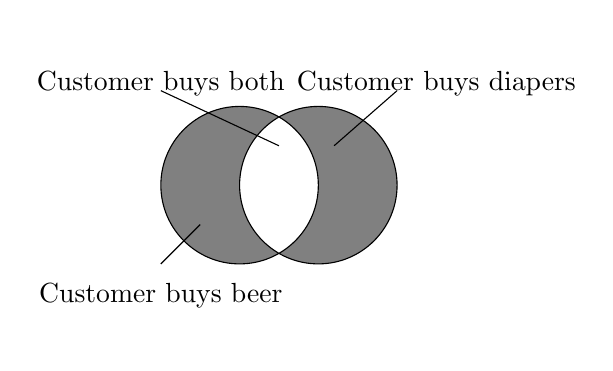
\begin{tikzpicture}[fill=gray]
          % left hand
          \scope
          \clip (-2,-2) rectangle (2,2)
                (1,0) circle (1);
          \fill (0,0) circle (1);
          \endscope
          % right hand
          \scope
          \clip (-2,-2) rectangle (2,2)
                (0,0) circle (1);
          \fill (1,0) circle (1);
          \endscope
          % outline
          \draw (0,0) circle (1) (0,1) (1,0) circle (1) (1,1);
          \node[label=below:{Customer buys beer}] at (-1,-1) {};
          \node[label=below:{Customer buys diapers}] at (2.5,1.7) {};
          \node[label=below:{Customer buys both}] at (-1,1.7) {};
          \draw (-1,-1) -- (-0.5,-0.5);
          \draw (2,1.2) -- (1.2,0.5);
          \draw (-1,1.2) -- (0.5,0.5);
          \end{tikzpicture}
          \end{column}
          \begin{column}{0.5\textwidth}
          \vspace{-2cm}
          \begin{itemize}
            \item \textbf{Itemset:}
            \begin{itemize}
              \item A set of one or more items.
              \item $k$-itemset $X = \{x_1, x_2, \ldots, x_k\}$.
            \end{itemize}
            \item \textbf{(Absolute) Support, or support count of $X$:}
            \begin{itemize}
              \item Frequency or occurrence of $X$.
            \end{itemize}
            \item (Relative) Support $s$:
            \begin{itemize}
              \item The fraction of the transactions that contain $X$.
              \item I.e. the \textbf{probability} that a transaction contains $X$.
            \end{itemize}
            \item \textbf{An itemset $X$ is frequent, if $X$'s support is no less than a \texttt{min\_sup} threshold.}
          \end{itemize}
          \end{column}
        \end{columns}
    \end{frame}
  }

  {
    \setbeamertemplate{footline}{}
    \begin{frame}{An example}
        \begin{columns}
          \begin{column}{0.4\textwidth}
          \begin{tabular}{|c|c|}
          \hline
          \textbf{TID} & \textbf{Items bought}\\\hline
          10 & Beer, Nuts, Diapers \\\hline
          20 & Beer, Coffee, Diapers \\\hline
          30 & Beer, Diapers, Eggs \\\hline
          40 & Nuts, Eggs, Milk \\\hline
          50 & Nuts, Coffee, Diapers, Eggs, Milk\\\hline
          \end{tabular}
          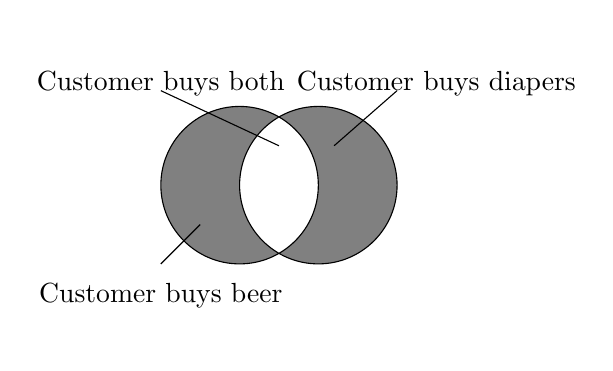
\begin{tikzpicture}[fill=gray]
          % left hand
          \scope
          \clip (-2,-2) rectangle (2,2)
                (1,0) circle (1);
          \fill (0,0) circle (1);
          \endscope
          % right hand
          \scope
          \clip (-2,-2) rectangle (2,2)
                (0,0) circle (1);
          \fill (1,0) circle (1);
          \endscope
          % outline
          \draw (0,0) circle (1) (0,1) (1,0) circle (1) (1,1);
          \node[label=below:{Customer buys beer}] at (-1,-1) {};
          \node[label=below:{Customer buys diapers}] at (2.5,1.7) {};
          \node[label=below:{Customer buys both}] at (-1,1.7) {};
          \draw (-1,-1) -- (-0.5,-0.5);
          \draw (2,1.2) -- (1.2,0.5);
          \draw (-1,1.2) -- (0.5,0.5);
          \end{tikzpicture}
          \end{column}
          \begin{column}{0.5\textwidth}
          \vspace{-2cm}
          \begin{itemize}
            \item \textbf{Find all the rules $X \implies Y$ with minimum support and confidence.}
            \begin{itemize}
              \item \textbf{Support} $s$: probability that a transaction contains $X \cup Y$.
              \item \textbf{Confidence} $c$: conditional probability that a transaction having $X$ also contains $Y$.
            \end{itemize}
            \item \textbf{Example:}
            \begin{itemize}
              \item Let $\text{min\_sup} = 50\%$ and $\text{min\_conf} = 50\%$.
              \item Frequent itemsets:
              \begin{itemize}
                \item Beer: $3$, Nuts: $3$,
                \item Diapers: $4$, Eggs: $3$,
                \item $\{\text{Beer, Diapers}\}$: $3$.
              \end{itemize}
              \item \textbf{Association rules:}
              \begin{itemize}
                \item Beer $\implies$ Diapers ($60\%$, $100\%$).
                \item Diapers $\implies$ Beer ($60\%$, $75\%$).
              \end{itemize}
            \end{itemize}
          \end{itemize}
          \end{column}
        \end{columns}
    \end{frame}
  }

  {
    \setbeamertemplate{footline}{}
    \begin{frame}{Basic concepts: association rules (2)}
    \begin{itemize}
      \item \textbf{Implication of the form $A \implies B$:}
      \begin{itemize}
        \item where $A \neq \emptyset$, $B \neq \emptyset$ and $A \cap B = \emptyset$.
      \end{itemize}
      \item \textbf{Strong rule:}
      \begin{itemize}
        \item Satisfies both $\text{min\_sup}$ and $\text{min\_conf}$
        \begin{align}
        \text{support}(A \implies B) &= P(A \cup B),\\
        \text{confidence}(A \implies B) &= P(B | A)\\
        &= \frac{\text{support}(A \cup B)}{\text{support}(A)}\\
        &= \frac{\text{support\_count}(A\cup B)}{\text{support\_count}(A)}.
        \end{align}
        \item I.e. confidence of rule can be easily derived from the support counts of $A$ and $A \cup B$.
      \end{itemize}
      \item \textbf{Association-rule mining:}
      \begin{itemize}
        \item Find all frequent itemsets.
        \item Generate strong association rules from the frequent itemsets.
      \end{itemize}
    \end{itemize}
    \end{frame}
  }

  {
    \setbeamertemplate{footline}{}
    \begin{frame}{Closed itemsets and max-itemsets}
    \begin{itemize}
      \item \textbf{A long itemset contains a combinatorial number of sub-itemsets.}
      \begin{itemize}
        \item E.g. $\{a_1,a_2,\ldots,a_{100}\}$ contains
        \begin{align}
        {100\choose 1} + {100 \choose 2} + \cdots + {100 \choose 100} = 2^{100}-1 \approx 1.27 \cdot 10^{30} \; \text{sub-itemsets!}
        \end{align}
        \item \textbf{Solution:}
        \begin{itemize}
          \item Mine closed itemsets and max-itemsets instead.
        \end{itemize}
        \item \textbf{An itemset $X$ is closed, if $X$ is frequent and there exists no super-itemset $X \subset Y$ with the same support as $X$.}
        \begin{itemize}
          \item Proposed by (Pasquier et al., ICDT'99).
        \end{itemize}
        \item \textbf{An itemset $X$ is a max-itemset, if $X$ is frequent and there exists no frequent super-itemset $X \subset Y$.}
        \begin{itemize}
          \item Proposed by (Bayardo, SIGMOD'98).
        \end{itemize}
        \item \textbf{Closed itemset is a lossless "compression" of frequent itemsets.}
        \begin{itemize}
          \item Reducing the number of itemsets (and rules).
        \end{itemize}
      \end{itemize}
    \end{itemize}
    \end{frame}
  }

  {
    \setbeamertemplate{footline}{}
    \begin{frame}{Closed itemsets and max-itemsets (II)}
    \begin{itemize}
      \item \textbf{Example:}
      \begin{itemize}
        \item $\text{DB} = \{\langle a_1,a_2, \ldots, a_{100} \rangle, \langle a_1, a_2, \ldots, a_{100} \rangle \}$.
        \item I.e. just two transactions.
        \item $\text{min\_sup} = 1$.
      \end{itemize}
      \item \textbf{What are the closed itemsets?}
      \begin{itemize}
        \item $\langle a_1,a_2, \ldots, a_{100} \rangle : 1$,
        \item $\langle a_1,a_2, \ldots, a_{50} \rangle : 2$,
        \item Number behind the colon: support\_count.
      \end{itemize}
      \item \textbf{What are the max-itemsets?}
      \begin{itemize}
        \item $\langle a_1,a_2, \ldots, a_{100} \rangle : 1$.
      \end{itemize}
      \item \textbf{What is the set of all frequent itemsets?}
    \end{itemize}
    \end{frame}
  }

  {
    \setbeamertemplate{footline}{}
    \begin{frame}{Chapter V: Mining frequent patterns, associations and correlations}
        \begin{itemize}
            \item Basic Concepts.
            \item \textbf{Scalable frequent-itemset-mining methods.}
            \begin{itemize}
              \item \textbf{Apriori: a candidate-generation-and-test approach.}
              \item Improving the efficiency of apriori.
              \item FPGrowth:  a frequent-pattern-growth approach.
              \item ECLAT: frequent-pattern mining with vertical data format.
              \item Mining closed itemsets and max-itemsets.
            \end{itemize}
            \item Generating association rules from frequent itemsets.
            \item Which patterns are interesting? Pattern-evaluation methods.
            \item Summary.
        \end{itemize}
    \end{frame}
  }

  {
    \setbeamertemplate{footline}{}
    \begin{frame}{The downward-closure property and scalable mining methods}
    \begin{itemize}
      \item \textbf{The downward-closure property of frequent patterns:}
      \begin{itemize}
        \item \textbf{\color{airforceblue}Any subset of a frequent itemset must also be frequent.}
        \begin{itemize}
          \item If $\{\text{Beer, Diapers, Nuts}\}$ is frequent, so is $\{\text{Beer, Diapers}\}$.
          \item I.e. every transaction having $\{\text{Beer, Diapers, Nuts}\}$ also contains $\{\text{Beer, Diapers}\}$.
        \end{itemize}
      \end{itemize}
      \item \textbf{Scalable mining methods: three major approaches.}
      \begin{itemize}
        \item A priori (Agrawal \& Srikant, VLDB'94).
        \item Frequent-pattern growth (FPgrowth) (Han, Pei \& Yin, SIGMOD'00).
        \item Vertical-data-format approach (CHARM) (Zaki \& Hsiao, SDM'02).
      \end{itemize}
    \end{itemize}
    \end{frame}
  }

  {
    \setbeamertemplate{footline}{}
    \begin{frame}{A priori: a candidate generation \& test approach}
    \begin{itemize}
      \item \textbf{A priori pruning principle:}
      \begin{itemize}
        \item \textbf{\color{airforceblue}If there is any itemset which is infrequent, \\ its supersets should not be generated/tested!} \\ (Agrawal \& Srikant, VLDB'94; Mannila et al., KDD'94)
      \end{itemize}
      \item \textbf{Method:}
      \begin{itemize}
        \item Initially, scan DB once to get frequent $1$-itemsets.
        \item Generate length-$(k+1)$ candidate itemsets from length-$k$ frequent itemsets.
        \item Test the candidates against DB, discard those that are infrequent.
        \item Terminate when no further candidate or frequent itemset can be generated.
      \end{itemize}
    \end{itemize}
    \end{frame}
  }

  {
    \setbeamertemplate{footline}{}
    \begin{frame}{A priori algorithm - an example}
    \centering
    \vspace{-0.7cm}
    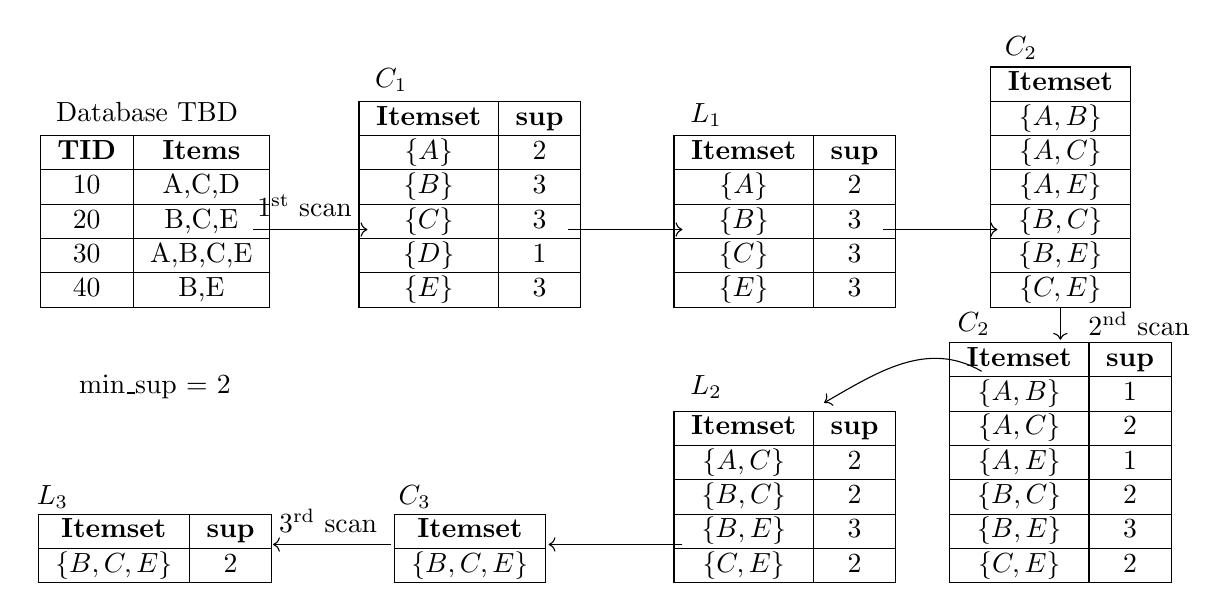
\begin{tikzpicture}
    \path (0,1) coordinate (A) node[above, inner sep=0] {
      \begin{tabular}{ | c | c |}
        \hline
        \textbf{TID} & \textbf{Items} \\\hline
        10 & A,C,D \\\hline
        20 & B,C,E \\\hline
        30 & A,B,C,E \\\hline
        40 & B,E \\\hline
      \end{tabular}
      };
    \path (4,1) coordinate (A) node[above, inner sep=0] {
      \begin{tabular}{ | c | c |}
        \hline
        \textbf{Itemset} & \textbf{sup} \\\hline
        $\{A\}$ & 2 \\\hline
        $\{B\}$ & 3 \\\hline
        $\{C\}$ & 3 \\\hline
        $\{D\}$ & 1 \\\hline
        $\{E\}$ & 3 \\\hline
      \end{tabular}
      };
    \path (8,1) coordinate (A) node[above, inner sep=0] {
      \begin{tabular}{ | c | c |}
        \hline
        \textbf{Itemset} & \textbf{sup} \\\hline
        $\{A\}$ & 2 \\\hline
        $\{B\}$ & 3 \\\hline
        $\{C\}$ & 3 \\\hline
        $\{E\}$ & 3 \\\hline
      \end{tabular}
      };
    \path (11.5,1) coordinate (A) node[above, inner sep=0] {
      \begin{tabular}{ | c |}
        \hline
        \textbf{Itemset} \\\hline
        $\{A,B\}$ \\\hline
        $\{A,C\}$ \\\hline
        $\{A,E\}$ \\\hline
        $\{B,C\}$ \\\hline
        $\{B,E\}$ \\\hline
        $\{C,E\}$ \\\hline
      \end{tabular}
      };
    \path (11.5,-2.5) coordinate (A) node[above, inner sep=0] {
      \begin{tabular}{ | c | c |}
        \hline
        \textbf{Itemset} & \textbf{sup} \\\hline
        $\{A,B\}$ & 1 \\\hline
        $\{A,C\}$ & 2 \\\hline
        $\{A,E\}$ & 1 \\\hline
        $\{B,C\}$ & 2 \\\hline
        $\{B,E\}$ & 3 \\\hline
        $\{C,E\}$ & 2 \\\hline
      \end{tabular}
      };
    \path (8,-2.5) coordinate (A) node[above, inner sep=0] {
      \begin{tabular}{ | c | c |}
        \hline
        \textbf{Itemset} & \textbf{sup} \\\hline
        $\{A,C\}$ & 2 \\\hline
        $\{B,C\}$ & 2 \\\hline
        $\{B,E\}$ & 3 \\\hline
        $\{C,E\}$ & 2 \\\hline
      \end{tabular}
      };
    \path (4,-2.5) coordinate (A) node[above, inner sep=0] {
      \begin{tabular}{ | c |}
        \hline
        \textbf{Itemset} \\\hline
        $\{B,C,E\}$ \\\hline
      \end{tabular}
      };
    \path (0,-2.5) coordinate (A) node[above, inner sep=0] {
      \begin{tabular}{ | c | c |}
        \hline
        \textbf{Itemset} & \textbf{sup} \\\hline
        $\{B,C,E\}$ & 2 \\\hline
      \end{tabular}
      };

    \draw[->] (1.25,2) -- (2.7,2);
    \draw[->] (5.25,2) -- (6.7,2);
    \draw[->] (9.25,2) -- (10.7,2);
    \draw[->] (10.5,0.2) to [out=150,in=30] (8.5,-0.2);
    \draw[->] (11.5,1) -- (11.5,0.6);
    \draw[->] (6.7,-2) -- (5,-2);
    \draw[->] (3,-2) -- (1.5,-2);
    \node at (-0.1,3.5) {Database TBD};
    \node at (1.9,2.3) {$1^{\text{st}}$ scan};
    \node at (2.2,-1.7) {$3^{\text{rd}}$ scan};
    \node at (12.5,0.8) {$2^{\text{nd}}$ scan};
    \node at (3,3.9) {$C_1$};
    \node at (7,3.45) {$L_1$};
    \node at (10.4,0.8) {$C_2$};
    \node at (11,4.3) {$C_2$};
    \node at (7,0) {$L_2$};
    \node at (3.3,-1.4) {$C_3$};
    \node at (-1.3,-1.4) {$L_3$};
    \node at (0,0) {min\_sup = 2};
    \end{tikzpicture}
    \end{frame}
  }

  {
    \setbeamertemplate{footline}{}
    \begin{frame}{A priori algorithm (pseudo code)}
    $C_k$: candidate itemsets of size $k$\\
    $L_k$: frequent itemsets of size $k$\\[0.5cm]

    $L_1 = \{\text{frequent items}\}$;\\[0.5cm]
    \textbf{for} $(k=1; L_k \neq \emptyset; k\texttt{++})$ \textbf{do begin}\\
    \hspace{1cm} $C_{k+1} = \text{candidates generated from } L_k;$\\
    \hspace{1cm} \textbf{for each} transaction $t$ in database \textbf{do}\\
    \hspace{2cm} increment the count of all candidates in $C_{k+1}$ that are contained in $t$;\\[0.1cm]
    \hspace{1cm}$L_{k+1} = \text{candidates in } C_{k+1} \text{ with min\_sup};$\\
    \textbf{end;}\\[0.1cm]
    \textbf{return} $\bigcup_k L_k$;
    \end{frame}
  }

  {
    \setbeamertemplate{footline}{}
    \begin{frame}{Implementation of a priori}
    \begin{itemize}
      \item \textbf{\color{airforceblue}How to generate candidates?}
      \begin{itemize}
        \item Step 1: self-joining $L_k$ (or joining $L_k$ with $L_1$).
        \item Step 2: pruning.
      \end{itemize}
      \item \textbf{Example of candidate generation:}
      \begin{itemize}
        \item $L_3 = \{abc, abd, acd, ace, bcd\}$.
        \item Self-joining: $L_3 \bowtie L_3$:
        \begin{itemize}
          \item $abcd$ from $abc$ and $abd$.
          \item $acde$ from $acd$ and $ace$.
        \end{itemize}
        \item \textbf{Pruning:}
        \begin{itemize}
          \item $acde$ is removed because $ade$ is not in $L_3$.
        \end{itemize}
        \item $C_4 = \{abcd\}$.
      \end{itemize}
    \end{itemize}
    \end{frame}
  }

  {
    \setbeamertemplate{footline}{}
    \begin{frame}{Implementation of a priori}
    \begin{itemize}
      \item \textbf{Why is counting supports of candidates a problem?}
      \begin{itemize}
        \item The total number of candidates can be huge.
        \item One transaction may contain many candidates.
      \end{itemize}
      \item \textbf{Method:}
      \begin{itemize}
        \item Candidate itemsets are stored in a \textbf{hash tree}.
        \item Leaf node of hash tree contains a list of itemsets and counts.
        \item Interior node contains a hash table.
        \item Subset function: finds all the candidates contained in a transaction.
      \end{itemize}
    \end{itemize}
    \end{frame}
  }

  {
    \setbeamertemplate{footline}{}
    \begin{frame}{Counting supports of candidates using hash tree}
    \centering
    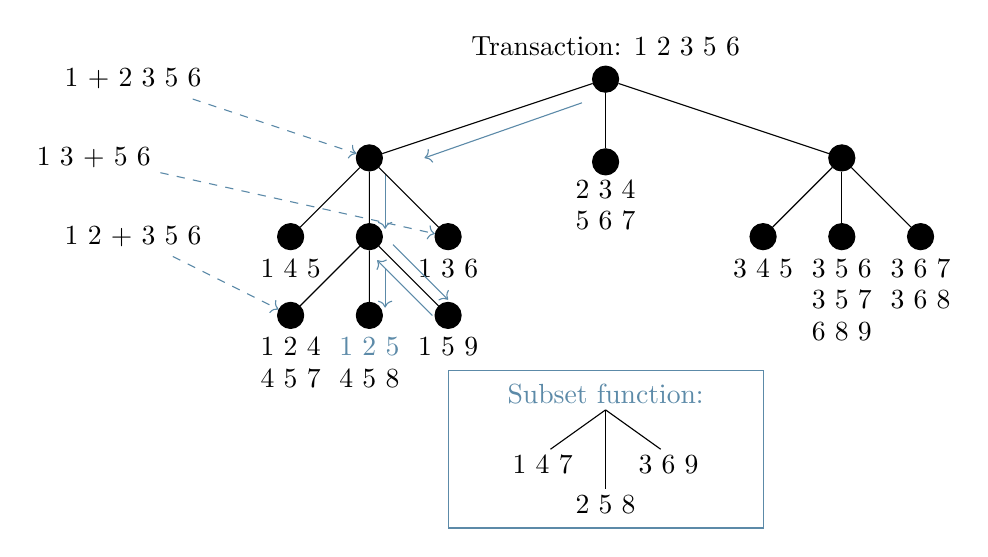
\begin{tikzpicture}
      \node[draw, circle, fill=black, label=above:{Transaction: 1 2 3 5 6}] (r) at (0,10) {};
      \draw[->, color=airforceblue] (-0.3,9.7) -- (-2.3,9);
      \node[draw, circle, fill=black] (a) at (0,8.95) {};
      \node at (0,8.6) {2 3 4};
      \node at (0,8.2) {5 6 7};
      \node[draw, circle, fill=black] (b) at (3,9) {};
      \node[draw, circle, fill=black] (c) at (-3,9) {};
      \node[draw, circle, fill=black] (d) at (-3,8) {};
      \node[draw, circle, fill=black] (e) at (-4,8) {};
      \node at (-4,7.6) {1 4 5};
      \node at (-6,10) (o) {1 + 2 3 5 6};
      \node at (-6.5,9) (p) {1 3 + 5 6};
      \node at (-6,8) (q) {1 2 + 3 5 6};
      \node[draw, circle, fill=black] (f) at (-2,8) {};
      \node at (-2,7.6) {1 3 6};
      \node[draw, circle, fill=black] (g) at (-3,7) {};
      \node at (-3,6.6) {\color{airforceblue}1 2 5};
      \node at (-3,6.2) {4 5 8};
      \node[draw, circle, fill=black] (h) at (-2,7) {};
      \node at (-2,6.6) {1 5 9};
      \node[draw, circle, fill=black] (i) at (-4,7) {};
      \node at (-4,6.6) {1 2 4};
      \node at (-4,6.2) {4 5 7};
      \draw[->, color=airforceblue] (-2.8, 7.6) -- (-2.8,7.1);
      \draw[->, color=airforceblue] (-2.8, 8.8) -- (-2.8,8.1);
      \draw[->, color=airforceblue] (-2.7, 7.9) -- (-2,7.2);
      \draw[->, color=airforceblue] (-2.2,7) -- (-2.9, 7.7);

      \node[draw, circle, fill=black] (j) at (3,8) {};
      \node at (3,7.6) {3 5 6};
      \node at (3,7.2) {3 5 7};
      \node at (3,6.8) {6 8 9};
      \node[draw, circle, fill=black] (k) at (4,8) {};
      \node at (4,7.6) {3 6 7};
      \node at (4,7.2) {3 6 8};
      \node[draw, circle, fill=black] (l) at (2,8) {};
      \node at (2,7.6) {3 4 5};

      \draw (r) -- (b);
      \draw (r) -- (a);
      \draw (r) -- (c) -- (d) -- (g);
      \draw (c) -- (e);
      \draw (c) -- (f);
      \draw (d) -- (h);
      \draw (d) -- (i);
      \draw (b) -- (j);
      \draw (b) -- (k);
      \draw (b) -- (l);
      \draw[->, dashed, color=airforceblue] (o) -- (c);
      \draw[->, dashed, color=airforceblue] (p) -- (f);
      \draw[->, dashed, color=airforceblue] (q) -- (i);

      \node at (0,6) {\color{airforceblue}Subset function:};
      \node at (-0.8,5.1) {1 4 7};
      \node at (0,4.6) {2 5 8};
      \node at (0.8,5.1) {3 6 9};
      \draw (-0.7,5.3) -- (0,5.8);
      \draw (0.7,5.3) -- (0,5.8);
      \draw (0,4.8) -- (0,5.8);
      \draw[color=airforceblue] (-2,6.3) -- (2,6.3) -- (2,4.3) -- (-2,4.3) -- (-2,6.3);
    \end{tikzpicture}
    \end{frame}
  }

  {
    \setbeamertemplate{footline}{}
    \begin{frame}{Candidate generation: an SQL implementation}
    \begin{itemize}
      \item \textbf{SQL implementation of candidate generation.}
      \begin{itemize}
        \item Suppose the items in $L_{k-1}$ are listed in order.
        \begin{itemize}
          \item[1.] Self-joining $L_{k-1}$.\\
                \texttt{INSERT INTO} $C_k$\\
                \hspace{1cm} (\texttt{SELECT p.item$_1$, p.item$_2$, $\ldots$, p.item$_{k-1}$, q.item$_{k-1}$}\\
                \hspace{1.1cm} \texttt{FROM $L_{k-1} p, L_{k-1} q$}\\
                \hspace{1.1cm} \texttt{WHERE p.item$_1$ = q.item$_1$, $\ldots$, p.item$_{k-2}$ = q.item$_{k-2}$, \\
                \hspace{2.05cm} p.item$_{k-1}$ $<$ q.item$_{k-1}$});
          \item[2.] Pruning.\\
                \hspace{1cm} \textbf{forall} itemsets $c$ in $C_k$ \textbf{do} \\
                \hspace{2cm} \textbf{forall} $(k-1)$-subsets $s$ of $c$ \textbf{do}\\
                \hspace{3cm} \textbf{if} ($s$ is not in $L_{k-1}$) \textbf{then} \texttt{DELETE} $c$ \texttt{FROM} $C_k$;
        \end{itemize}
        \item \textbf{Use object-relational extensions like UDFs, BLOBs, and table functions for efficient implementation.}
        \begin{itemize}
          \item (Sarawagi, Thomas \& Agrawal, SIGMOD'98)
        \end{itemize}
      \end{itemize}
    \end{itemize}
    \end{frame}
  }

  {
    \setbeamertemplate{footline}{}
    \begin{frame}{Chapter V: Mining frequent patterns, associations and correlations}
        \begin{itemize}
            \item Basic Concepts.
            \item Scalable frequent-itemset-mining methods.
            \begin{itemize}
              \item Apriori: a candidate-generation-and-test approach.
              \item \textbf{Improving the efficiency of apriori.}
              \item FPGrowth:  a frequent-pattern-growth approach.
              \item ECLAT: frequent-pattern mining with vertical data format.
              \item Mining closed itemsets and max-itemsets.
            \end{itemize}
            \item Generating association rules from frequent itemsets.
            \item Which patterns are interesting? Pattern-evaluation methods.
            \item Summary.
        \end{itemize}
    \end{frame}
  }

  {
    \setbeamertemplate{footline}{}
    \begin{frame}{Further improvement of the a priori method}
        \begin{itemize}
            \item \textbf{Major computational challenges.}
              \begin{itemize}
                \item Multiple scans of transaction database.
                \item Huge number of candidates.
                \item Tedious workload of support counting for candidates.
              \end{itemize}
            \item \textbf{Improving a priori: general ideas.}
              \begin{itemize}
              \item Reduce passes of transaction-database scans.
              \item Shrink number of candidates.
              \item Facilitate support counting of candidates.
              \end{itemize}
        \end{itemize}
    \end{frame}
  }

  {
    \setbeamertemplate{footline}{}
    \begin{frame}{Hashing: reduce the number of candidates}
    \begin{columns}
      \begin{column}{0.6\textwidth}
      \begin{itemize}
        \item \textbf{A $k$-itemset whose corresponding hashing-bucket count is below the threshold cannot be frequent.}
        \begin{itemize}
          \item Candidates: $a,b,c,d,e$.
          \item While scanning DB for frequent $1$-itemsets, create hash entries for $2$-itemsets:
          \begin{itemize}
            \item $\{ab,ad,ae\}$
            \item $\{bd,be,de\}$
            \item $\ldots$
          \end{itemize}
          \item Frequent $1$-itemset: $a,b,d,e$.
          \item $ab$ is not a candidate $2$-itemset, if the sum of count of $\{ab, ad, ae\}$ is below support threshold.
          \item (Park, Chen \& Yu, SIGMOD'95)
        \end{itemize}
      \end{itemize}
      \end{column}
      \begin{column}{0.3\textwidth}
      \centering
      \textbf{Hash table:}\\
      \begin{tabular}{| c | c |}
      \hline
      count & itemsets \\\hline
      35 & $\{ab,ad,ae\}$\\\hline
      88 & $\{bd,be,de\}$\\\hline
      $\vdots$ & $\vdots$\\\hline
      102 & $\{yz,qs,wt\}$\\\hline
      \end{tabular}
      \end{column}
    \end{columns}
    \end{frame}
  }

  {
    \setbeamertemplate{footline}{}
    \begin{frame}{Partition: scan database only twice}
    \begin{itemize}
      \item \textbf{Any itemset that is potentially frequent in DB must be frequent in at least one of the partitions of DB.}
      \begin{itemize}
        \item Scan 1: partition database and find local frequent patterns:
        \begin{itemize}
          \item $\text{min\_sup}_i = \text{min\_sup}[\%] \cdot \vert \text{DB}_i \vert$.
        \end{itemize}
        \item Scan 2: consolidate global frequent patterns.\\
              (Savasere, Omiecinski \& Navathe, VLDB'95)
      \end{itemize}
      \vspace{0.5cm}
    \end{itemize}
    \centering
    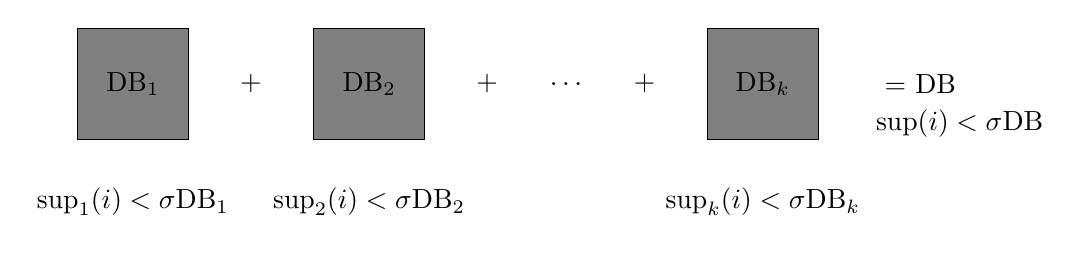
\begin{tikzpicture}[square/.style={regular polygon,regular polygon sides=4}]
    \node at (0,0) [square, draw, fill=gray, minimum size=2cm] {};
    \node at (3,0) [square, draw, fill=gray, minimum size=2cm] {};
    \node at (8,0) [square, draw, fill=gray, minimum size=2cm] {};
    \node at (5.5,0) {$\hdots$};
    \node at (0,0) {DB$_1$};
    \node at (0,-1.5) {$\sup_1(i) < \sigma \text{DB}_1$};
    \node at (3,-1.5) {$\sup_2(i) < \sigma \text{DB}_2$};
    \node at (8,-1.5) {$\sup_k(i) < \sigma \text{DB}_k$};
    \node at (10.5,-0.5) {$\sup(i) < \sigma \text{DB}$};
    \node at (3,0) {DB$_2$};
    \node at (8,0) {DB$_k$};
    \node at (4.5,0) {+};
    \node at (6.5,0) {+};
    \node at (1.5,0) {+};
    \node at (10,0) {= DB};
    \end{tikzpicture}
    \end{frame}
  }

  {
    \setbeamertemplate{footline}{}
    \begin{frame}{Sampling for frequent patterns}
    \begin{itemize}
      \item \textbf{Select a sample of original database,\\
       mine frequent patterns within sample using a priori.}
      \item \textbf{Scan database once to verify frequent itemsets found in sample,\\
       only {\color{airforceblue}borders} of closure of frequent patterns are checked.}
      \begin{itemize}
        \item Example: check $abcd$ instead of $ab, ac, \ldots,$ etc.
      \end{itemize}
      \item \textbf{Scan database again to find missed frequent patterns.}\\
      (Toivonen, VLDB'96)
    \end{itemize}
    \end{frame}
  }

  {
    \setbeamertemplate{footline}{}
    \begin{frame}{Dynamic itemset counting: reduce number of scans}
    \begin{itemize}
      \item \textbf{Adding candidate itemsets at different points during a scan.}
      \begin{itemize}
        \item DB partitioned into blocks marked by \textbf{\color{airforceblue}start points}.
        \item New candidate itemsets can be added at any start point during a scan.
        \begin{itemize}
            \item E.g. if $A$ and $B$ are already found to be frequent, \\
            $AB$ are also counted from that starting point on.
        \end{itemize}
        \item Uses the count-so-far as the lower bound of the actual count.
        \item If count-so-far passes minimum support, itemset is added to frequent-itemset collection.
        \item Can then be used to generate even longer candidates.
      \end{itemize}
    \end{itemize}
    \end{frame}
  }

  {
    \setbeamertemplate{footline}{}
    \begin{frame}{Dynamic itemset counting: reduce number of scans (II)}
    \begin{columns}
    \begin{column}{0.5\textwidth}
    \centering
    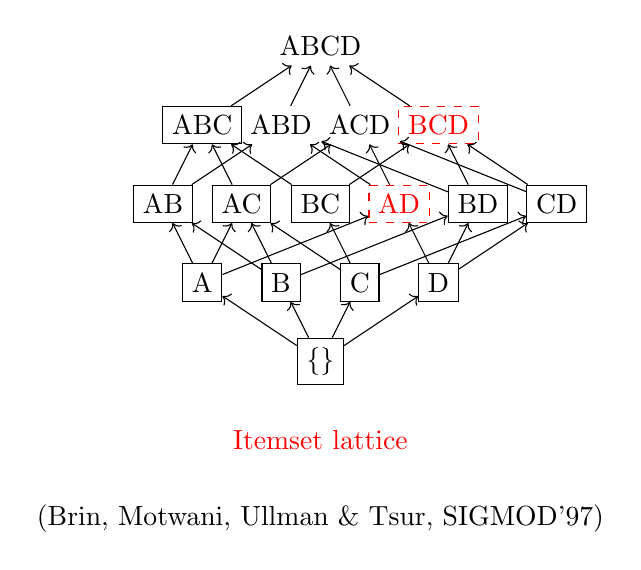
\begin{tikzpicture}
    \node at (0,0) (abcd) {ABCD};
    \node[draw] at (-1.5,-1) (abc) {ABC};
    \node at (-0.5,-1) (abd) {ABD};
    \node at (0.5,-1) (acd) {ACD};
    \node[draw, dashed, color=red] at (1.5,-1) (bcd) {BCD};

    \node[draw] at (-2,-2) (ab) {AB};
    \node[draw] at (-1,-2) (ac) {AC};
    \node[draw] at (0,-2) (bc) {BC};
    \node[draw, dashed, color=red] at (1,-2) (ad) {AD};
    \node[draw] at (2,-2) (bd) {BD};
    \node[draw] at (3,-2) (cd) {CD};

    \node[draw] at (-1.5,-3) (a) {A};
    \node[draw] at (-0.5,-3) (b) {B};
    \node[draw] at (0.5,-3) (c) {C};
    \node[draw] at (1.5,-3) (d) {D};
    \node[draw] at (0,-4) (0) {$\{\}$};
    \node at (0,-5) {\color{red}Itemset lattice};
    \node at (0,-6) {(Brin, Motwani, Ullman \& Tsur, SIGMOD'97)};

    \draw[->] (0)-- (a);
    \draw[->] (0)-- (b);
    \draw[->] (0)-- (c);
    \draw[->] (0)-- (d);
    \draw[->] (a)-- (ab);
    \draw[->] (a)-- (ac);
    \draw[->] (a)-- (ad);
    \draw[->] (b)-- (ab);
    \draw[->] (b)-- (ac);
    \draw[->] (b)-- (bd);
    \draw[->] (c)-- (ac);
    \draw[->] (c)-- (bc);
    \draw[->] (c)-- (cd);
    \draw[->] (d)-- (ad);
    \draw[->] (d)-- (bd);
    \draw[->] (d)-- (cd);

    \draw[->] (ab)-- (abc);
    \draw[->] (ab)-- (abd);
    \draw[->] (ac)-- (abc);
    \draw[->] (ac)-- (acd);
    \draw[->] (bc)-- (abc);
    \draw[->] (bc)-- (bcd);
    \draw[->] (ad)-- (abd);
    \draw[->] (ad)-- (acd);
    \draw[->] (bd)-- (abd);
    \draw[->] (bd)-- (bcd);
    \draw[->] (cd)-- (acd);
    \draw[->] (cd)-- (bcd);

    \draw[->] (abc)-- (abcd);
    \draw[->] (abd)-- (abcd);
    \draw[->] (acd)-- (abcd);
    \draw[->] (bcd)-- (abcd);
    \end{tikzpicture}
    \end{column}
    \begin{column}{0.5\textwidth}
    \vspace{-6.5cm}
    \begin{itemize}
      \item Once both $A$ and $D$ are determined frequent,\\
      the counting of $AD$ begins.
      \item Once length-$2$ subsets of $BCD$ are determined frequent, the counting of $BCD$ begins.
    \end{itemize}
    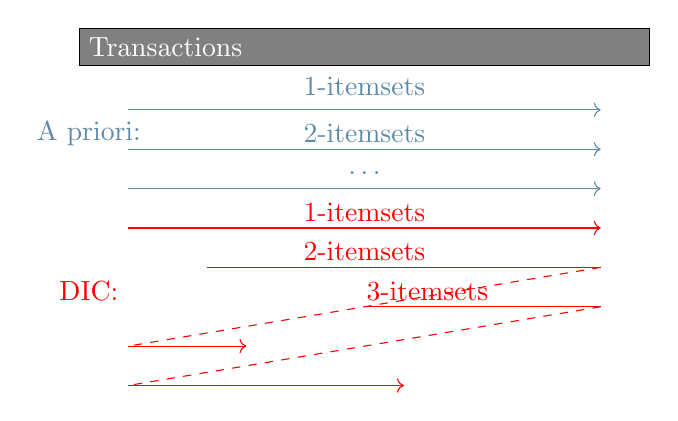
\begin{tikzpicture}
    \node[draw, fill=gray, text width = 7cm] {\color{white}Transactions};
    \draw[->, color=airforceblue] (-3,-0.8) -- (3,-0.8);
    \draw[->, color=airforceblue] (-3,-1.3) -- (3,-1.3);
    \draw[->, color=airforceblue] (-3,-1.8) -- (3,-1.8);
    \draw[->, color=red] (-3,-2.3) -- (3,-2.3);
    \draw[color=red] (-2,-2.8) -- (3,-2.8);
    \draw[color=red] (0,-3.3) -- (3,-3.3);
    \draw[->, color=red] (-3,-3.8) -- (-1.5,-3.8);
    \draw[->, color=red] (-3,-4.3) -- (0.5,-4.3);
    \node at (0, -0.5) {\color{airforceblue}1-itemsets};
    \node at (0, -1.1) {\color{airforceblue}2-itemsets};
    \node at (0, -2.1) {\color{red}1-itemsets};
    \node at (0, -2.6) {\color{red}2-itemsets};
    \node at (0.8, -3.1) {\color{red}3-itemsets};
    \node at (0, -1.6) {\color{airforceblue}$\ldots$};
    \draw[dashed, color=red] (3,-2.8) -- (-3,-3.8);
    \draw[dashed, color=red] (3,-3.3) -- (-3,-4.3);
    \node at (-3.5, -3.1) {\color{red}DIC:};
    \node at (-3.5, -1.1) {\color{airforceblue}A priori:};
    \end{tikzpicture}
    \end{column}
    \end{columns}
    \end{frame}
  }

  {
    \setbeamertemplate{footline}{}
    \begin{frame}{Chapter V: Mining frequent patterns, associations and correlations}
        \begin{itemize}
            \item Basic Concepts.
            \item Scalable frequent-itemset-mining methods.
            \begin{itemize}
              \item Apriori: a candidate-generation-and-test approach.
              \item Improving the efficiency of apriori.
              \item \textbf{FPGrowth:  a frequent-pattern-growth approach.}
              \item ECLAT: frequent-pattern mining with vertical data format.
              \item Mining closed itemsets and max-itemsets.
            \end{itemize}
            \item Generating association rules from frequent itemsets.
            \item Which patterns are interesting? Pattern-evaluation methods.
            \item Summary.
        \end{itemize}
    \end{frame}
  }

 {
    \setbeamertemplate{footline}{}
    \begin{frame}{Pattern-growth approach: mining frequent patterns without candidate generation}
        \begin{itemize}
            \item \textbf{Bottlenecks of the a priori approach.}
            \begin{itemize}
                \item Breadth-first (i.e., level-wise) search.
                \item Candidate generation and test.
                \begin{itemize}
                    \item Often generates a huge number of candidates.
                \end{itemize}
            \end{itemize}
            \item \textbf{The FPGrowth Approach.} (Han, Pei \& Yin, SIGMOD'00)
            \begin{itemize}
                \item Depth-first search.
                \item Avoid explicit candidate generation.
            \end{itemize}
            \item \textbf{Major philosophy: Grow long patterns from short ones using local frequent items only.}
            \begin{itemize}
                \item $abc$ is a frequent pattern.
                \item Get all transactions having $abc$, i.e. restrict DB on $abc$: $DB|_{abc}$.
                \item $d$ is a local frequent item in $DB|_{abc \implies abcd}$ is a frequent pattern.
            \end{itemize}
        \end{itemize}
    \end{frame}
  }

  {
    \setbeamertemplate{footline}{}
    \begin{frame}{Construct FP-tree from a transaction database}
    \centering
    \begin{tabular}{|c|c|c|}
    \hline
    \underline{TID} & \underline{Items bought} & \underline{(ordered) frequent items} \\\hline
    100 & $\{f,a,c,d,g,i,m,p\}$ & $\{f,c,a,m,p\}$ \\\hline
    200 & $\{a,b,c,f,l,m,p\}$ & $\{f,c,a,b,m\}$ \\\hline
    300 & $\{b,f,h,j,o,w\}$ & $\{f,b\}$ \\\hline
    400 & $\{b,c,k,s,p\}$ & $\{c,b,p\}$ \\\hline
    500 & $\{a,f,c,e,l,p,m,n\}$ & $\{f,c,a,m,p\}$ \\\hline
    \end{tabular}
    \vspace{0.2cm}
    \begin{columns}
    \begin{column}{0.5\textwidth}
    \vspace{-3.5cm}
    \begin{itemize}
      \item[1.] Scan DB once, find frequent $1$-itemsets (single-item patterns).
      \item[2.] Sort frequent items in frequency-descending order, creating the \textbf{f-list}.
      \item[3.] Scan DB again, construct \textbf{FP-tree}.
    \end{itemize}
    \end{column}
    \begin{column}{0.5\textwidth}
    \centering
    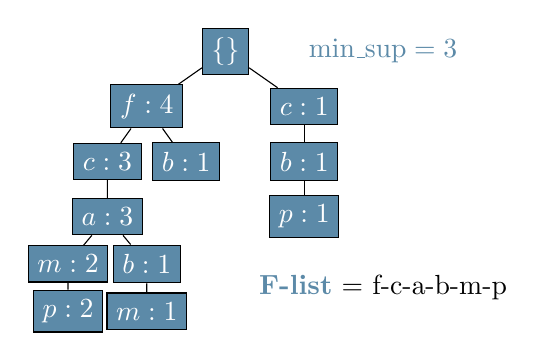
\begin{tikzpicture}
    \node[draw, fill=airforceblue] at (0,0) (0) {\color{white}$\{\}$};
    \node[draw, fill=airforceblue] at (-1,-0.7) (f4) {\color{white}$f:4$};
    \node[draw, fill=airforceblue] at (-1.5,-1.4) (c3) {\color{white}$c:3$};
    \node[draw, fill=airforceblue] at (-1.5,-2.1) (a3) {\color{white}$a:3$};
    \node[draw, fill=airforceblue] at (-2,-2.7) (m2) {\color{white}$m:2$};
    \node[draw, fill=airforceblue] at (-2,-3.3) (p2) {\color{white}$p:2$};
    \node[draw, fill=airforceblue] at (-1,-2.7) (b12) {\color{white}$b:1$};
    \node[draw, fill=airforceblue] at (-1,-3.3) (m1) {\color{white}$m:1$};

    \node[draw, fill=airforceblue] at (-0.5,-1.4) (b1) {\color{white}$b:1$};
    \node[draw, fill=airforceblue] at (1,-0.7) (c1) {\color{white}$c:1$};
    \node[draw, fill=airforceblue] at (1,-1.4) (b13) {\color{white}$b:1$};
    \node[draw, fill=airforceblue] at (1,-2.1) (p1) {\color{white}$p:1$};
    \draw (0) -- (f4) -- (c3) -- (a3) -- (m2) -- (p2);
    \draw (0) -- (c1);
    \draw (f4) -- (b1);
    \draw (a3) -- (b12) -- (m1);
    \draw (c1) -- (b13) -- (p1);
    \node at (2,0) (0) {\color{airforceblue}$\text{min\_sup}=3$};
    \node at (2,-3) (0) {\textbf{\color{airforceblue}F-list} = f-c-a-b-m-p};
    \end{tikzpicture}
    \end{column}
    \end{columns}
    \end{frame}
  }

  {
    \setbeamertemplate{footline}{}
    \begin{frame}{Partition itemsets and databases}
    \begin{itemize}
      \item \textbf{Frequent itemsets can be partitioned into subsets according to f-list.}
      \begin{itemize}
        \item F-list = f-c-a-b-m-p.
        \item Patterns containing p.
        \begin{itemize}
          \item The least-frequent item (at the end of the f-list, suffix).
        \end{itemize}
        \item Patterns having m but not p.
        \item $\vdots$
        \item Patterns having c but not a nor b, m, p.
        \item Pattern f.
      \end{itemize}
      \item \textbf{This processing order guarantees completeness and non-redundancy.}
    \end{itemize}
    \end{frame}
  }

  {
    \setbeamertemplate{footline}{}
    \begin{frame}{Find itemsets having item $p$ from $p$'s conditional pattern base}
    \begin{itemize}
      \item \textbf{Starting at the frequent-item header table in the FP-tree.}
      \item \textbf{Traverse the FP-tree by following the link of frequent item $p$.}
      \item \textbf{Accumulate all transformed {\color{airforceblue}prefix paths} of item $p$ to form $p$'s {\color{red}conditional pattern base}.}
    \end{itemize}
    \vspace{0.2cm}
    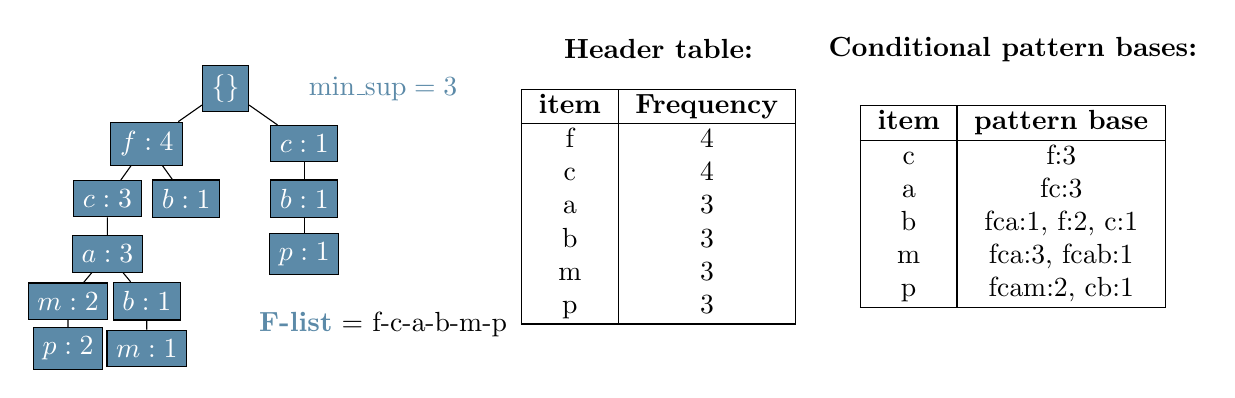
\begin{tikzpicture}
    \node[draw, fill=airforceblue] at (0,0) (0) {\color{white}$\{\}$};
    \node[draw, fill=airforceblue] at (-1,-0.7) (f4) {\color{white}$f:4$};
    \node[draw, fill=airforceblue] at (-1.5,-1.4) (c3) {\color{white}$c:3$};
    \node[draw, fill=airforceblue] at (-1.5,-2.1) (a3) {\color{white}$a:3$};
    \node[draw, fill=airforceblue] at (-2,-2.7) (m2) {\color{white}$m:2$};
    \node[draw, fill=airforceblue] at (-2,-3.3) (p2) {\color{white}$p:2$};
    \node[draw, fill=airforceblue] at (-1,-2.7) (b12) {\color{white}$b:1$};
    \node[draw, fill=airforceblue] at (-1,-3.3) (m1) {\color{white}$m:1$};

    \node[draw, fill=airforceblue] at (-0.5,-1.4) (b1) {\color{white}$b:1$};
    \node[draw, fill=airforceblue] at (1,-0.7) (c1) {\color{white}$c:1$};
    \node[draw, fill=airforceblue] at (1,-1.4) (b13) {\color{white}$b:1$};
    \node[draw, fill=airforceblue] at (1,-2.1) (p1) {\color{white}$p:1$};
    \draw (0) -- (f4) -- (c3) -- (a3) -- (m2) -- (p2);
    \draw (0) -- (c1);
    \draw (f4) -- (b1);
    \draw (a3) -- (b12) -- (m1);
    \draw (c1) -- (b13) -- (p1);
    \node at (2,0) (0) {\color{airforceblue}$\text{min\_sup}=3$};
    \node at (2,-3) (0) {\textbf{\color{airforceblue}F-list} = f-c-a-b-m-p};
    \node at (5.5,0.5) (0) {\textbf{Header table:}};
    \node at (10,0.5) (0) {\textbf{Conditional pattern bases:}};
    \node at (5.5,-1.5) (0) {
    \begin{tabular}{|c|c|}
    \hline
    \textbf{item} & \textbf{Frequency} \\\hline
    f & 4 \\
    c & 4 \\
    a & 3 \\
    b & 3 \\
    m & 3 \\
    p & 3 \\\hline
    \end{tabular}
    };
    \node at (10,-1.5) (0) {
    \begin{tabular}{|c|c|}
    \hline
    \textbf{item} & \textbf{pattern base} \\\hline
    c & f:3 \\
    a & fc:3 \\
    b & fca:1, f:2, c:1 \\
    m & fca:3, fcab:1 \\
    p & fcam:2, cb:1 \\
    \hline
    \end{tabular}
    };
    \end{tikzpicture}
    \end{frame}
  }

  {
    \setbeamertemplate{footline}{}
    \begin{frame}{$p$'s conditional pattern base}
    \centering
    \begin{tikzpicture}
    \node[draw, fill=airforceblue] at (0,0) (0) {\color{white}$\{\}$};
    \node[draw, fill=ForestGreen] at (-1,-0.7) (f2) {\color{white}$f:2$};
    \node[draw, fill=ForestGreen] at (-1.5,-1.4) (c2) {\color{white}$c:2$};
    \node[draw, fill=ForestGreen] at (-1.5,-2.1) (a2) {\color{white}$a:2$};
    \node[draw, fill=ForestGreen] at (-2,-2.7) (m2) {\color{white}$m:2$};
    \node[draw, fill=red] at (-2,-3.3) (p2) {\color{white}$p:2$};
    \node[draw, fill=airforceblue] at (-1,-2.7) (b12) {\color{white}$b:1$};
    \node[draw, fill=airforceblue] at (-1,-3.3) (m1) {\color{white}$m:1$};

    \node[draw, fill=airforceblue] at (-0.5,-1.4) (b1) {\color{white}$b:1$};
    \node[draw, fill=ForestGreen] at (1,-0.7) (c1) {\color{white}$c:1$};
    \node[draw, fill=ForestGreen] at (1,-1.4) (b13) {\color{white}$b:1$};
    \node[draw, fill=red] at (1,-2.1) (p1) {\color{white}$p:1$};
    \draw (0) -- (f4) -- (c3) -- (a3) -- (m2) -- (p2);
    \draw (0) -- (c1);
    \draw (f4) -- (b1);
    \draw (a3) -- (b12) -- (m1);
    \draw (c1) -- (b13) -- (p1);
    \node at (5.5,0.5) (0) {\textbf{Header table:}};
    \node at (5.5,-1.5) (0) {
    \begin{tabular}{|c|c|}
    \hline
    \textbf{item} & \textbf{Frequency} \\\hline
    f & 4 \\
    c & 4 \\
    a & 3 \\
    b & 3 \\
    m & 3 \\
    \textbf{\color{red}p} & \textbf{\color{red}3} \\\hline
    \end{tabular}
    };
    \end{tikzpicture}\\[0.2cm]
    Hence, $p$'s conditional pattern base is\\
    fcam:2, cb:1\\
    both below min\_sup.
    \end{frame}
  }

  {
    \setbeamertemplate{footline}{}
    \begin{frame}{$m$'s conditional pattern base}
    \centering
    \begin{tikzpicture}
    \node[draw, fill=airforceblue] at (0,0) (0) {\color{white}$\{\}$};
    \node[draw, fill=ForestGreen] at (-1,-0.7) (f2) {\color{white}$f:3$};
    \node[draw, fill=ForestGreen] at (-1.5,-1.4) (c2) {\color{white}$c:3$};
    \node[draw, fill=ForestGreen] at (-1.5,-2.1) (a2) {\color{white}$a:3$};
    \node[draw, fill=red] at (-2,-2.7) (m2) {\color{white}$m:2$};
    \node[draw, fill=airforceblue] at (-2,-3.3) (p2) {\color{white}$p:2$};
    \node[draw, fill=ForestGreen] at (-1,-2.7) (b12) {\color{white}$b:1$};
    \node[draw, fill=red] at (-1,-3.3) (m1) {\color{white}$m:1$};

    \node[draw, fill=airforceblue] at (-0.5,-1.4) (b1) {\color{white}$b:1$};
    \node[draw, fill=airforceblue] at (1,-0.7) (c1) {\color{white}$c:1$};
    \node[draw, fill=airforceblue] at (1,-1.4) (b13) {\color{white}$b:1$};
    \node[draw, fill=airforceblue] at (1,-2.1) (p1) {\color{white}$p:1$};
    \draw (0) -- (f4) -- (c3) -- (a3) -- (m2) -- (p2);
    \draw (0) -- (c1);
    \draw (f4) -- (b1);
    \draw (a3) -- (b12) -- (m1);
    \draw (c1) -- (b13) -- (p1);
    \node at (5.5,0.5) (0) {\textbf{Header table:}};
    \node at (5.5,-1.5) (0) {
    \begin{tabular}{|c|c|}
    \hline
    \textbf{item} & \textbf{Frequency} \\\hline
    f & 4 \\
    c & 4 \\
    a & 3 \\
    b & 3 \\
    \textbf{\color{red}m} & \textbf{\color{red}3} \\
    p & 3 \\\hline
    \end{tabular}
    };
    \end{tikzpicture}\\[0.2cm]
    Hence, $m$'s conditional pattern base is\\
    fca:3, fcab:1\\
    {\color{ForestGreen}fca has min\_sup.}
    \end{frame}
  }

  {
    \setbeamertemplate{footline}{}
    \begin{frame}{$b$'s conditional pattern base}
    \centering
    \begin{tikzpicture}
    \node[draw, fill=airforceblue] at (0,0) (0) {\color{white}$\{\}$};
    \node[draw, fill=ForestGreen] at (-1,-0.7) (f2) {\color{white}$f:2$};
    \node[draw, fill=ForestGreen] at (-1.5,-1.4) (c2) {\color{white}$c:1$};
    \node[draw, fill=ForestGreen] at (-1.5,-2.1) (a2) {\color{white}$a:1$};
    \node[draw, fill=airforceblue] at (-2,-2.7) (m2) {\color{white}$m:2$};
    \node[draw, fill=airforceblue] at (-2,-3.3) (p2) {\color{white}$p:2$};
    \node[draw, fill=red] at (-1,-2.7) (b12) {\color{white}$b:1$};
    \node[draw, fill=airforceblue] at (-1,-3.3) (m1) {\color{white}$m:1$};

    \node[draw, fill=red] at (-0.5,-1.4) (b1) {\color{white}$b:1$};
    \node[draw, fill=ForestGreen] at (1,-0.7) (c1) {\color{white}$c:1$};
    \node[draw, fill=red] at (1,-1.4) (b13) {\color{white}$b:1$};
    \node[draw, fill=airforceblue] at (1,-2.1) (p1) {\color{white}$p:1$};
    \draw (0) -- (f4) -- (c3) -- (a3) -- (m2) -- (p2);
    \draw (0) -- (c1);
    \draw (f4) -- (b1);
    \draw (a3) -- (b12) -- (m1);
    \draw (c1) -- (b13) -- (p1);
    \node at (5.5,0.5) (0) {\textbf{Header table:}};
    \node at (5.5,-1.5) (0) {
    \begin{tabular}{|c|c|}
    \hline
    \textbf{item} & \textbf{Frequency} \\\hline
    f & 4 \\
    c & 4 \\
    a & 3 \\
    \textbf{\color{red}b} & \textbf{\color{red}3} \\
    m & 3 \\
    p & 3 \\\hline
    \end{tabular}
    };
    \end{tikzpicture}\\[0.2cm]
    Hence, $b$'s conditional pattern base is\\
    fca:1, f:2, c:1\\
    {all below min\_sup.}
    \end{frame}
  }

  {
    \setbeamertemplate{footline}{}
    \begin{frame}{$a$'s conditional pattern base}
    \centering
    \begin{tikzpicture}
    \node[draw, fill=airforceblue] at (0,0) (0) {\color{white}$\{\}$};
    \node[draw, fill=ForestGreen] at (-1,-0.7) (f2) {\color{white}$f:3$};
    \node[draw, fill=ForestGreen] at (-1.5,-1.4) (c2) {\color{white}$c:3$};
    \node[draw, fill=red] at (-1.5,-2.1) (a2) {\color{white}$a:3$};
    \node[draw, fill=airforceblue] at (-2,-2.7) (m2) {\color{white}$m:2$};
    \node[draw, fill=airforceblue] at (-2,-3.3) (p2) {\color{white}$p:2$};
    \node[draw, fill=airforceblue] at (-1,-2.7) (b12) {\color{white}$b:1$};
    \node[draw, fill=airforceblue] at (-1,-3.3) (m1) {\color{white}$m:1$};

    \node[draw, fill=airforceblue] at (-0.5,-1.4) (b1) {\color{white}$b:1$};
    \node[draw, fill=airforceblue] at (1,-0.7) (c1) {\color{white}$c:1$};
    \node[draw, fill=airforceblue] at (1,-1.4) (b13) {\color{white}$b:1$};
    \node[draw, fill=airforceblue] at (1,-2.1) (p1) {\color{white}$p:1$};
    \draw (0) -- (f4) -- (c3) -- (a3) -- (m2) -- (p2);
    \draw (0) -- (c1);
    \draw (f4) -- (b1);
    \draw (a3) -- (b12) -- (m1);
    \draw (c1) -- (b13) -- (p1);
    \node at (5.5,0.5) (0) {\textbf{Header table:}};
    \node at (5.5,-1.5) (0) {
    \begin{tabular}{|c|c|}
    \hline
    \textbf{item} & \textbf{Frequency} \\\hline
    f & 4 \\
    c & 4 \\
    \textbf{\color{red}a} & \textbf{\color{red}3} \\
    b & 3 \\
    m & 3 \\
    p & 3 \\\hline
    \end{tabular}
    };
    \end{tikzpicture}\\[0.2cm]
    Hence, $a$'s conditional pattern base is\\
    fc:3\\
    {has min\_sup.}
    \end{frame}
  }

  {
    \setbeamertemplate{footline}{}
    \begin{frame}{From conditional pattern bases to conditional FP-trees }
    \centering
    \begin{itemize}
      \item \textbf{For each conditional pattern base:}
      \begin{itemize}
        \item Accumulate the count for each item in the base.
        \item Construct the conditional FP-tree for the frequent items of the pattern base.
      \end{itemize}
    \end{itemize}
    \begin{tikzpicture}
    \node[draw, fill=airforceblue] at (0,0) (0) {\color{white}$\{\}$};
    \node[draw, fill=airforceblue] at (-1,-0.7) (f2) {\color{white}$f:3$};
    \node[draw, fill=airforceblue] at (-1.5,-1.4) (c2) {\color{white}$c:3$};
    \node[draw, fill=airforceblue] at (-1.5,-2.1) (a2) {\color{white}$a:3$};
    \node[draw, fill=airforceblue] at (-2,-2.7) (m2) {\color{white}$m:2$};
    \node[draw, fill=airforceblue] at (-2,-3.3) (p2) {\color{white}$p:2$};
    \node[draw, fill=airforceblue] at (-1,-2.7) (b12) {\color{white}$b:1$};
    \node[draw, fill=airforceblue] at (-1,-3.3) (m1) {\color{white}$m:1$};

    \node[draw, fill=airforceblue] at (-0.5,-1.4) (b1) {\color{white}$b:1$};
    \node[draw, fill=airforceblue] at (1,-0.7) (c1) {\color{white}$c:1$};
    \node[draw, fill=airforceblue] at (1,-1.4) (b13) {\color{white}$b:1$};
    \node[draw, fill=airforceblue] at (1,-2.1) (p1) {\color{white}$p:1$};
    \draw (0) -- (f4) -- (c3) -- (a3) -- (m2) -- (p2);
    \draw (0) -- (c1);
    \draw (f4) -- (b1);
    \draw (a3) -- (b12) -- (m1);
    \draw (c1) -- (b13) -- (p1);
    \node at (5.5,-3.5) {\textbf{All frequent patterns related to $m$:}};
    \node at (5.5,-4) {m, fm, cm, am, fcm, fam, cam, fcam;};
    \node at (10,-1) (10) {$\{\}$};
    \node at (10,-2) (11) {$f:3$};
    \node at (10,-3) (12) {$c:3$};
    \node at (10,-4) (13) {$a:3$};
    \node at (10,0.5) {$m$'s conditional pattern base:};
    \node at (10,0) {fca:3, fcab:1;};
    \node at (10,-0.5) {$m$'s conditional FP-tree:};
    \draw (10) -- (11) -- (12) -- (13);
    \node at (5.5,0.5) {\textbf{Header table:}};
    \node at (5.5,-1.5) {
    \begin{tabular}{|c|c|}
    \hline
    \textbf{item} & \textbf{Frequency} \\\hline
    f & 4 \\
    c & 4 \\
    a & 3 \\
    b & 3 \\
    m & 3 \\
    p & 3 \\\hline
    \end{tabular}
    };
    \end{tikzpicture}
    \end{frame}
  }

  {
    \setbeamertemplate{footline}{}
    \begin{frame}{Recursion: mining each conditional FP-tree}
    \centering
    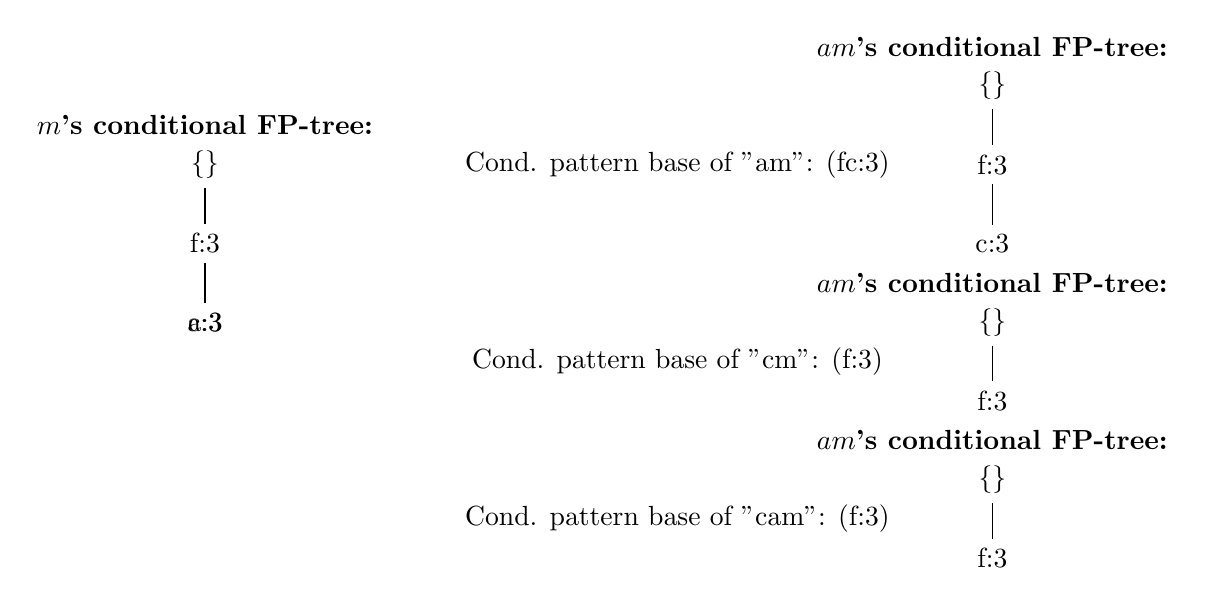
\begin{tikzpicture}
      \node at (0,0.5) (0) {\textbf{$m$'s conditional FP-tree:}};
      \node at (0,0) (0) {$\{\}$};
      \node at (0,-1) (f3) {f:3};
      \node at (0,-2) (c3) {c:3};
      \node at (0,-2) (a3) {a:3};
      \draw (0)--(f3)--(c3)--(a3);

      \node at (6,-0) (r0) {Cond. pattern base of "am": (fc:3)};
      \node at (6,-2.5) (r0) {Cond. pattern base of "cm": (f:3)};
      \node at (6,-4.5) (r0) {Cond. pattern base of "cam": (f:3)};

      \node at (10,1.5) (0) {\textbf{$am$'s conditional FP-tree:}};
      \node at (10,1) (r0) {$\{\}$};
      \node at (10,0) (rf3) {f:3};
      \node at (10,-1) (rc3) {c:3};
      \draw (r0)--(rf3)--(rc3);

      \node at (10,-1.5) (0) {\textbf{$am$'s conditional FP-tree:}};
      \node at (10,-2) (rr0) {$\{\}$};
      \node at (10,-3) (rrf3) {f:3};
      \draw (rr0)--(rrf3);

      \node at (10,-3.5) (0) {\textbf{$am$'s conditional FP-tree:}};
      \node at (10,-4) (rrr0) {$\{\}$};
      \node at (10,-5) (rrrf3) {f:3};
      \draw (rrr0)--(rrrf3);
    \end{tikzpicture}
    \end{frame}
  }

  {
    \setbeamertemplate{footline}{}
    \begin{frame}{A special case: single prefix path in FP-tree}
    \centering
    \begin{itemize}
      \item \textbf{Suppose a (conditional) FP-tree $T$ has a shared single prefix-path $P$.}
      \item Mining can be decomposed into two parts.
      \begin{itemize}
        \item Reduction of the single prefix path into one node.
        \item Concatenation of the mining results of the two parts.
      \end{itemize}
    \end{itemize}
    \centering
    \begin{tikzpicture}
      \node at (0,0) (0) {$\{\}$};
      \node at (0,-0.7) (a1n1) {$a_1:n_1$};
      \node at (0,-1.4) (a2n2) {$a_2:n_2$};
      \node at (0,-2.1) (a3n3) {$a_3:n_3$};
      \node at (-0.7,-2.8) (b1m1) {$b_1:m_1$};
      \node at (0.7,-2.8) (c1k1) {$c_1:k_1$};
      \node at (0,-3.5) (c2k2) {$c_2:k_2$};
      \node at (1.4,-3.5) (c3k3) {$c_3:k_3$};
      \draw (0)--(a1n1)--(a2n2)--(a3n3)--(b1m1);
      \draw (a3n3)--(c1k1);
      \draw (c1k1)--(c2k2);
      \draw (c1k1)--(c3k3);
      \node at (2.1,-2.1) (join) {$\bowtie$};
      \node at (3.5,-2.1) (r1) {$r_1$};
      \node at (4,-2.1) (r1) {$=$};
      \node at (5,0) (20) {$\{\}$};
      \node at (5,-0.7) (2a1n1) {$a_1:n_1$};
      \node at (5,-1.4) (2a2n2) {$a_2:n_2$};
      \node at (5,-2.1) (2a3n3) {$a_3:n_3$};
      \draw (20)--(2a1n1)--(2a2n2)--(2a3n3);
      \node at (7,-2.1) (r1) {$+$};
      \node at (8.4,-2.1) (30) {$r_1$};
      \node at (8.1,-2.8) (b1m1) {$b_1:m_1$};
      \node at (9.5,-2.8) (c1k1) {$c_1:k_1$};
      \node at (8.4,-3.5) (c2k2) {$c_2:k_2$};
      \node at (9.9,-3.5) (c3k3) {$c_3:k_3$};
      \draw (30)--(c1k1)--(c3k3);
      \draw (30)--(b1m1);
      \draw (c1k1)--(c2k2);
    \end{tikzpicture}
    \end{frame}
  }

  {
    \setbeamertemplate{footline}{}
    \begin{frame}{A special case: single prefix path in FP-tree}
    \centering
    \begin{itemize}
      \item \textbf{Completeness.}
      \begin{itemize}
        \item Preserve complete information for frequent-pattern mining.
        \item Never break a long pattern of any transaction.
      \end{itemize}
      \item \textbf{Compactness.}
      \begin{itemize}
        \item Reduce irrelevant info - infrequent items are gone.
        \item Items in frequency-descending order.
        \begin{itemize}
          \item The more frequently occurring, the more likely to be shared.
        \end{itemize}
        \item Never larger than the original database.
        \begin{itemize}
          \item Not counting node links and the count fields.
        \end{itemize}
      \end{itemize}
    \end{itemize}
    \end{frame}
  }

  {
    \setbeamertemplate{footline}{}
    \begin{frame}{The frequent-pattern-growth mining method}
    \centering
    \begin{itemize}
      \item \textbf{Idea: Frequent-pattern growth.}
      \begin{itemize}
        \item Recursively grow frequent patterns by pattern and database partition.
      \end{itemize}
      \item \textbf{Method:}
      \begin{itemize}
        \item For each frequent item, construct its conditional pattern base, \\
        and then its conditional FP-tree.
        \item Repeat the process on each newly created conditional FP-tree.
        \item Until the resulting FP-tree is empty, or it contains only one path.
        \begin{itemize}
          \item Single path will generate all the combinations of its sub-paths, \\
          each of which is a frequent pattern.
        \end{itemize}
      \end{itemize}
    \end{itemize}
    \end{frame}
  }

  {
    \setbeamertemplate{footline}{}
    \begin{frame}{Scaling FP-growth by database projection}
    \centering
    \begin{itemize}
      \item \textbf{What if FP-tree does not fit in memory?}
      \begin{itemize}
        \item DB projection.
      \end{itemize}
      \item \textbf{First partition database into a set of projected DBs.}
      \item \textbf{Then construct and mine FP-tree for each projected DB.}
      \item \textbf{Parallel-projection vs. partition-projection techniques:}
      \begin{itemize}
        \item \textbf{\color{airforceblue}Parallel projection:}
        \begin{itemize}
          \item Project the DB in parallel for each frequent item.
          \item Parallel projection is space costly.
          \item All the partitions can be processed in parallel.
        \end{itemize}
        \item \textbf{\color{airforceblue}Partition projection:}
        \begin{itemize}
          \item Partition the DB based on the ordered frequent items.
          \item Passing the unprocessed parts to the subsequent partitions.
        \end{itemize}
      \end{itemize}
    \end{itemize}
    \end{frame}
  }

  {
    \setbeamertemplate{footline}{}
    \begin{frame}{Partition-based projection}
    \centering
    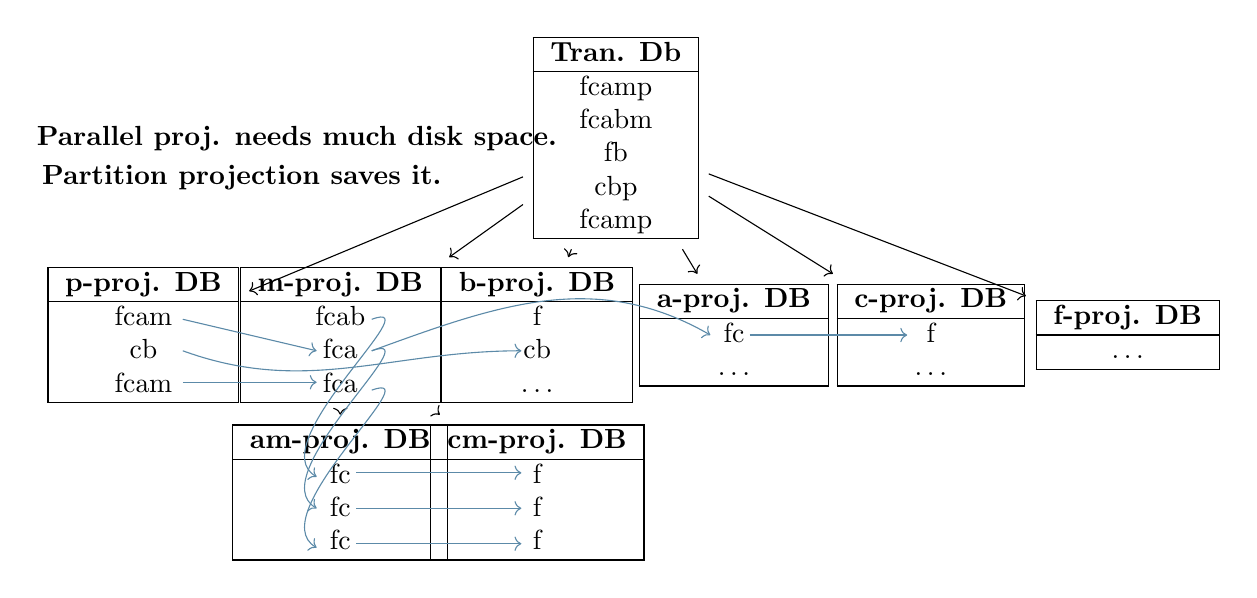
\begin{tikzpicture}
      \node at (-4.05,0) {\textbf{Parallel proj. needs much disk space.}};
      \node at (-4.75,-0.5) {\textbf{Partition projection saves it.}};
      \node at (0,-0) (0) {
      \begin{tabular}{|c|}
      \hline
      \textbf{Tran. Db}\\\hline
      fcamp \\
      fcabm \\
      fb \\
      cbp \\
      fcamp\\\hline
      \end{tabular}
      };
      \node at (-6,-2.5) (1) {
      \begin{tabular}{|c|}
      \hline
      \textbf{p-proj. DB}\\\hline
      fcam \\
      cb \\
      fcam \\\hline
      \end{tabular}
      };
      \node at (-3.5,-2.5) (2) {
      \begin{tabular}{|c|}
      \hline
      \textbf{m-proj. DB}\\\hline
      fcab \\
      fca \\
      fca \\\hline
      \end{tabular}
      };
      \node at (-1,-2.5) (3) {
      \begin{tabular}{|c|}
      \hline
      \textbf{b-proj. DB}\\\hline
      f \\
      cb \\
      $\ldots$ \\\hline
      \end{tabular}
      };
      \node at (1.5,-2.5) (4) {
      \begin{tabular}{|c|}
      \hline
      \textbf{a-proj. DB}\\\hline
      fc \\
      $\ldots$ \\\hline
      \end{tabular}
      };
      \node at (4,-2.5) (5) {
      \begin{tabular}{|c|}
      \hline
      \textbf{c-proj. DB}\\\hline
      f \\
      $\ldots$ \\\hline
      \end{tabular}
      };
      \node at (6.5,-2.5) (6) {
      \begin{tabular}{|c|}
      \hline
      \textbf{f-proj. DB}\\\hline
      $\ldots$ \\\hline
      \end{tabular}
      };
      \node at (-3.5,-4.5) (10) {
      \begin{tabular}{|c|}
      \hline
      \textbf{am-proj. DB}\\\hline
      fc \\
      fc \\
      fc \\\hline
      \end{tabular}
      };
      \node at (-1,-4.5) (11) {
      \begin{tabular}{|c|}
      \hline
      \textbf{cm-proj. DB}\\\hline
      f \\
      f \\
      f \\\hline
      \end{tabular}
      };
      \draw[->] (0)--(1);
      \draw[->] (0)--(2);
      \draw[->] (0)--(3);
      \draw[->] (0)--(4);
      \draw[->] (0)--(5);
      \draw[->] (0)--(6);
      \draw[->] (2)--(10);
      \draw[->] (2)--(11);
      \draw[->, color=airforceblue] (-5.5,-2.3) -- (-3.8,-2.7);
      \draw[->, color=airforceblue] (-5.5,-3.1) -- (-3.8,-3.1);
      \draw[->, color=airforceblue] (-5.5,-2.7) to [out=-20,in=-180] (-1.2,-2.7);
      \draw[->, color=airforceblue] (-3.1,-2.3) to [out=20,in=-210] (-3.8,-4.3);
      \draw[->, color=airforceblue] (-3.1,-2.7) to [out=20,in=-210] (-3.8,-4.7);
      \draw[->, color=airforceblue] (-3.1,-2.7) to [out=20,in=-210] (1.2,-2.5);
      \draw[->, color=airforceblue] (1.7,-2.5) -- (3.7,-2.5);
      \draw[->, color=airforceblue] (-3.1,-3.2) to [out=20,in=-210] (-3.8,-5.2);
      \draw[->, color=airforceblue] (-3.3,-5.15) -- (-1.2,-5.15);
      \draw[->, color=airforceblue] (-3.3,-4.7) -- (-1.2,-4.7);
      \draw[->, color=airforceblue] (-3.3,-4.25) -- (-1.2,-4.25);
    \end{tikzpicture}
    \end{frame}
  }

  {
    \setbeamertemplate{footline}{}
    \begin{frame}{Advantages of the pattern-growth approach}
    \begin{itemize}
      \item \textbf{Divide-and-conquer:}
      \begin{itemize}
        \item Decompose both the mining task and DB according \\
         to the frequent patterns obtained so far.
        \item Leading to focused search of smaller databases.
      \end{itemize}
      \item \textbf{Other factors:}
      \begin{itemize}
        \item No candidate generation, no candidate test.
        \item Compressed database: FP-tree structure.
        \item No repeated scan of entire database.
        \item Basic ops: counting local frequent items and building sub FP-tree,\\
        no pattern search and matching.
      \end{itemize}
      \item \textbf{A good open-source implementation and refinement of FP-growth:}
      \begin{itemize}
        \item FPGrowth+ (Grahne \& Zhu, FIMI'03)
      \end{itemize}
    \end{itemize}
    \end{frame}
  }

  {
    \setbeamertemplate{footline}{}
    \begin{frame}{Further improvements of mining methods}
    \begin{itemize}
      \item \textbf{AFOPT} (Liu et al., KDD'03)
      \begin{itemize}
        \item A "push-right" method for mining condensed frequent-pattern (CFP) tree.
      \end{itemize}
      \item \textbf{Carpenter} (Pan et al., KDD'03)
      \begin{itemize}
        \item Mine datasets with small rows but numerous columns.
        \item Construct a row-enumeration tree for efficient mining.
      \end{itemize}
      \item \textbf{FPgrowth+} (Grahne \& Zhu, FIMI'03)
      \begin{itemize}
        \item Efficiently using prefix-trees in mining frequent itemsets.
      \end{itemize}
      \item \textbf{TD-Close} (Liu et al., SDM'06)
    \end{itemize}
    \end{frame}
  }

  {
    \setbeamertemplate{footline}{}
    \begin{frame}{Extension of pattern-growth mining methodology }
    \begin{itemize}
      \item \textbf{Mining closed frequent itemsets and max-patterns.}
      \begin{itemize}
        \item CLOSET (DMKD'00), FPclose, and FPMax (Grahne \& Zhu, FIMI'03)
      \end{itemize}
      \item \textbf{Mining sequential patterns.}
      \begin{itemize}
        \item PrefixSpan (ICDE'01), CloSpan (SDM'03), BIDE (ICDE'04)
      \end{itemize}
      \item \textbf{Mining graph patterns.}
      \begin{itemize}
        \item gSpan (ICDM'02), CloseGraph (KDD'03)
      \end{itemize}
      \item \textbf{Constraint-based mining of frequent patterns.}
      \begin{itemize}
        \item Convertible constraints (ICDE'01), gPrune (PAKDD'03)
      \end{itemize}
      \item \textbf{Computing iceberg data cubes with complex measures.}
      \begin{itemize}
        \item H-tree, H-cubing, and Star-cubing (SIGMOD'01, VLDB'03)
      \end{itemize}
      \item \textbf{Pattern-growth-based clustering.}
      \begin{itemize}
        \item MaPle (Pei et al., ICDM'03)
      \end{itemize}
      \item \textbf{Pattern-growth-based classification.}
      \begin{itemize}
        \item Mining frequent and discriminative patterns (Cheng et al., ICDE'07)
      \end{itemize}
    \end{itemize}
    \end{frame}
  }

  {
    \setbeamertemplate{footline}{}
    \begin{frame}{Chapter V: Mining frequent patterns, associations and correlations}
        \begin{itemize}
            \item Basic Concepts.
            \item Scalable frequent-itemset-mining methods.
            \begin{itemize}
              \item Apriori: a candidate-generation-and-test approach.
              \item Improving the efficiency of apriori.
              \item FPGrowth:  a frequent-pattern-growth approach.
              \item \textbf{ECLAT: frequent-pattern mining with vertical data format.}
              \item Mining closed itemsets and max-itemsets.
            \end{itemize}
            \item Generating association rules from frequent itemsets.
            \item Which patterns are interesting? Pattern-evaluation methods.
            \item Summary.
        \end{itemize}
    \end{frame}
  }

  {
    \setbeamertemplate{footline}{}
    \begin{frame}{ECLAT: mining by exploring vertical data format}
        \begin{itemize}
            \item \textbf{Vertical format: $t(AB) = \{T_{11},T_{25},\ldots\}$}
            \begin{itemize}
              \item Tid-list: list of transaction ids containing an itemset.
            \end{itemize}
            \item \textbf{Deriving frequent itemsets based on vertical intersections.}
            \begin{itemize}
              \item $t(X) = t(Y): X$ and $Y$ always happen together.
              \item $t(X) \implies t(Y):$ transaction having $X$ always has $Y$.
            \end{itemize}
            \item \textbf{Using diffset to accelerate mining.}
            \begin{itemize}
              \item Only keep track of differences of tids.
              \item $t(X) = \{T_1,T_2,T_3\}$, $t(XY) = \{T_1,T_3\}$.
              \item Diffset $(XY,X) = \{T_2\}$.
            \end{itemize}
            \item \textbf{ECLAT} (Zaki et al., KDD'97)
            \item \textbf{Mining closed itemsets using vertical format: CHARM} (Zaki \& Hsiao, SDM'02)
        \end{itemize}
    \end{frame}
  }

  {
    \setbeamertemplate{footline}{}
    \begin{frame}{Chapter V: Mining frequent patterns, associations and correlations}
        \begin{itemize}
            \item Basic Concepts.
            \item Scalable frequent-itemset-mining methods.
            \begin{itemize}
              \item Apriori: a candidate-generation-and-test approach.
              \item Improving the efficiency of apriori.
              \item FPGrowth:  a frequent-pattern-growth approach.
              \item ECLAT: frequent-pattern mining with vertical data format.
              \item \textbf{Mining closed itemsets and max-itemsets.}
            \end{itemize}
            \item Generating association rules from frequent itemsets.
            \item Which patterns are interesting? Pattern-evaluation methods.
            \item Summary.
        \end{itemize}
    \end{frame}
  }

  {
    \setbeamertemplate{footline}{}
    \begin{frame}{Mining closed itemsets: CLOSET}
      \begin{columns}
        \begin{column}{0.6\textwidth}
        \begin{itemize}
            \item \textbf{Flist: list of all frequent items \\ in support-ascending order.}
            \begin{itemize}
              \item Flist: d-a-f-e-c.
            \end{itemize}
            \item \textbf{Divide search space.}
            \begin{itemize}
              \item Itemsets having d.
              \item Itemsets having d but not a, etc.
            \end{itemize}
            \item \textbf{Find closed itemsets recursively.}
            \begin{itemize}
              \item Every transaction having d also has $cfa \implies cfad$ is a closed itemset.
              \item (Pei, Han \& Mao, DMKD'00)
            \end{itemize}
        \end{itemize}
      \end{column}
      \begin{column}{0.3\textwidth}
        $\text{min\_sup} =2$ \\[0.2cm]
        \begin{tabular}{|c|c|}
          \hline
          TID & Items \\\hline
          10 & a,c,d,e,f \\\hline
          20 & a,b,e \\\hline
          30 & c,e,f \\\hline
          40 & a,c,d,f \\\hline
          50 & c,e,f \\\hline
        \end{tabular}
      \end{column}
      \end{columns}
    \end{frame}
  }

  {
    \setbeamertemplate{footline}{}
    \begin{frame}{Mining closed itemsets: CLOSET}
        \begin{itemize}
            \item \textbf{Itemset merging:.}
            \begin{itemize}
              \item If $Y$ appears in each occurrence of $X$, then $Y$ is merged with $X$.
            \end{itemize}
            \item \textbf{Sub-itemset pruning:}
            \begin{itemize}
              \item If $X \subset Y$ and $\text{sup}(X) = \text{sup}(Y),$ $X$ and all of $X$'s\\
              descendants in the set enumeration tree can be pruned.
            \end{itemize}
            \item \textbf{Hybrid tree projection:}
            \begin{itemize}
              \item Bottom-up physical tree projection.
              \item Top-down pseudo tree projection.
            \end{itemize}
            \item \textbf{Item skipping:}
            \begin{itemize}
              \item If a local frequent item has the same support in several header tables at different levels, \\
              one can prune it from the header table at higher levels.
            \end{itemize}
            \item \textbf{Efficient subset checking.}
        \end{itemize}
    \end{frame}
  }

  {
    \setbeamertemplate{footline}{}
    \begin{frame}{MaxMiner: mining max-itemsets}
      \begin{columns}
        \begin{column}{0.6\textwidth}
        \begin{itemize}
            \item \textbf{1st scan: find frequent items.}
            \begin{itemize}
              \item A, B, C, D, E
            \end{itemize}
            \item \textbf{2nd scan: find support for:}
            \begin{itemize}
              \item AB, AC, AD, AE, \textbf{ABCDE}
              \item BC, BD, BE, \textbf{BCDE}
              \item CD, CE, \textbf{CDE}, DE
            \end{itemize}
            \item \textbf{Potential max-itemsets: ABCDE, BCDE, CDE.}
            \item \textbf{Since BCDE is a max-itemset, no need to check BCD, BDE, CDE in later scan.} (Bayardo, SIGMOD'98)
        \end{itemize}
      \end{column}
      \begin{column}{0.3\textwidth}
        \begin{tabular}{|c|c|}
          \hline
          TID & Items \\\hline
          10 & A,B,C,D,E \\\hline
          20 & B,C,D,E \\\hline
          30 & A,C,D,F \\\hline
        \end{tabular}
      \end{column}
      \end{columns}
    \end{frame}
  }

  {
    \setbeamertemplate{footline}{}
    \begin{frame}{Chapter V: Mining frequent patterns, associations and correlations}
        \begin{itemize}
            \item Basic Concepts.
            \item Scalable frequent-itemset-mining methods.
            \begin{itemize}
              \item Apriori: a candidate-generation-and-test approach.
              \item Improving the efficiency of apriori.
              \item FPGrowth:  a frequent-pattern-growth approach.
              \item ECLAT: frequent-pattern mining with vertical data format.
              \item Mining closed itemsets and max-itemsets.
            \end{itemize}
            \item \textbf{Generating association rules from frequent itemsets.}
            \item Which patterns are interesting? Pattern-evaluation methods.
            \item Summary.
        \end{itemize}
    \end{frame}
  }

  {
    \setbeamertemplate{footline}{}
    \begin{frame}{Generating association rules from frequent itemsets}
        \begin{itemize}
            \item \textbf{Once frequent itemsets from transactions in database $D$ found:}
            \begin{itemize}
              \item Generate strong association rules from them,\\
                    Where "strong" = satisfying both minimum support and minimum confidence.
                    \begin{align}
                      \text{confidence}(A \implies B) &= P(B|A)\\
                      &= \frac{\text{support}(A \implies B)}{\text{support}(A)}\\
                      &= \frac{\text{support\_count}(A \implies B)}{\text{support\_count}(A)}
                    \end{align}
            \end{itemize}
            \item \textbf{For each frequent itemset $l$:}
            \begin{itemize}
              \item Generate all \textbf{nonempty subsets} of $l$.
            \end{itemize}
            \item \textbf{For every $s$ in $l$:}
            \begin{itemize}
              \item Output the rule $s \implies (l - s)$, if
              \item min\_sup is satisfied, because only frequent itemsets used.
            \end{itemize}
        \end{itemize}
    \end{frame}
  }

  {
    \setbeamertemplate{footline}{}
    \begin{frame}{Visualization of association rules: plane graph}
    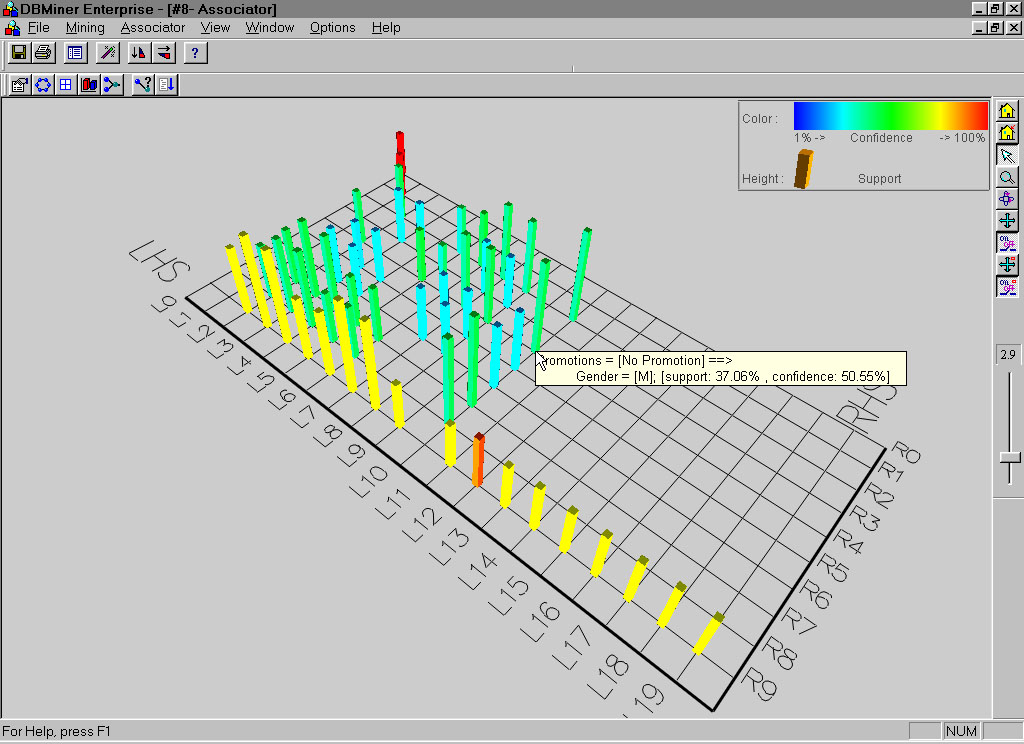
\includegraphics[width=0.6\textwidth]{img/assoc_rules1.jpg}
    \end{frame}
  }

  {
    \setbeamertemplate{footline}{}
    \begin{frame}{Visualization of association rules: rule graph}
    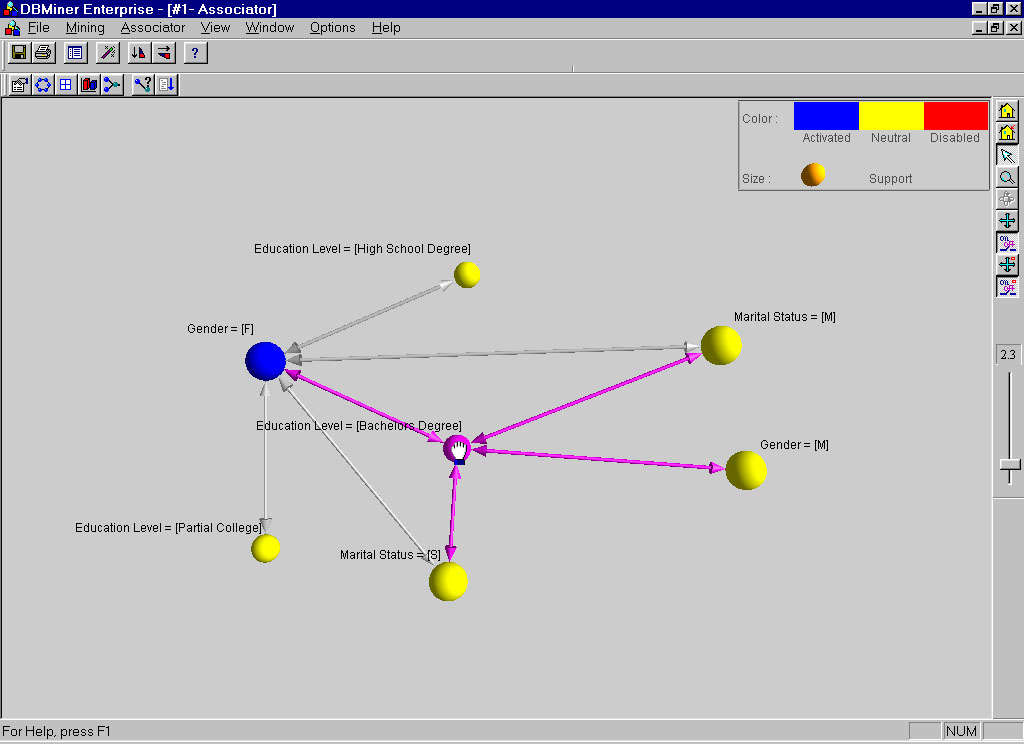
\includegraphics[width=0.6\textwidth]{img/assoc_rules2.jpg}
    \end{frame}
  }

  {
    \setbeamertemplate{footline}{}
    \begin{frame}{Visualization of association rules: SGI/MineSet 3.0}
    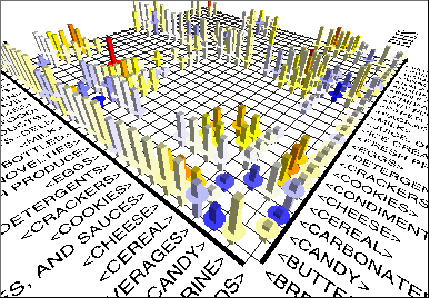
\includegraphics[width=0.6\textwidth]{img/assoc_rules3.png}
    \end{frame}
  }

  {
    \setbeamertemplate{footline}{}
    \begin{frame}{Chapter V: Mining frequent patterns, associations and correlations}
        \begin{itemize}
            \item Basic Concepts.
            \item Scalable frequent-itemset-mining methods.
            \begin{itemize}
              \item Apriori: a candidate-generation-and-test approach.
              \item Improving the efficiency of apriori.
              \item FPGrowth:  a frequent-pattern-growth approach.
              \item ECLAT: frequent-pattern mining with vertical data format.
              \item Mining closed itemsets and max-itemsets.
            \end{itemize}
            \item Generating association rules from frequent itemsets.
            \item \textbf{Which patterns are interesting? Pattern-evaluation methods.}
            \item Summary.
        \end{itemize}
    \end{frame}
  }

  {
    \setbeamertemplate{footline}{}
    \begin{frame}{Chapter V: Mining frequent patterns, associations and correlations}
        \begin{itemize}
            \item Basic Concepts.
            \item Scalable frequent-itemset-mining methods.
            \begin{itemize}
              \item Apriori: a candidate-generation-and-test approach.
              \item Improving the efficiency of apriori.
              \item FPGrowth:  a frequent-pattern-growth approach.
              \item ECLAT: frequent-pattern mining with vertical data format.
              \item Mining closed itemsets and max-itemsets.
            \end{itemize}
            \item Generating association rules from frequent itemsets.
            \item Which patterns are interesting? Pattern-evaluation methods.
            \item \textbf{Summary.}
        \end{itemize}
    \end{frame}
  }

  {
    \setbeamertemplate{footline}{}
    \begin{frame}{Summary}
        \begin{itemize}
          \item \textbf{Basic concepts:}
          \begin{itemize}
            \item Association rules.
            \item Support-confidence framework.
            \item Closed and max-itemsets.
          \end{itemize}
          \item \textbf{Scalable frequent-itemset-mining methods:}
          \begin{itemize}
            \item A priori:
            \begin{itemize}
              \item Candidate generation \& test.
            \end{itemize}
            \item Projection-based:
            \begin{itemize}
              \item FPgrowth, CLOSET+, $\ldots$
            \end{itemize}
            \item Vertical-format approach:
            \begin{itemize}
              \item ECLAT, CHARM, $\ldots$
            \end{itemize}
          \end{itemize}
          \item \textbf{Association rules generated from frequent itemsets.}
          \item \textbf{Which patterns are interesting?}
          \begin{itemize}
            \item Pattern-evaluation methods.
          \end{itemize}
        \end{itemize}
    \end{frame}
  }

  {
    \setbeamertemplate{footline}{}
    \begin{frame}{Interestingness measure: correlation (lift)}
        \begin{itemize}
          \item \textbf{(play) basketball $\implies$ (eat) cereal ($40\%$, $66.7\%$)  misleading:}
          \begin{itemize}
            \item The overall $\%$ of students eating cereal is $75\% > 66.7\%$.
          \end{itemize}
          \item \textbf{basketball $\implies$ no cereal ($20\%$, $33.3\%$)  more accurate:}
          \begin{itemize}
            \item Although with lower support and confidence.
          \end{itemize}
          \item \textbf{Reason: negative correlation.}
          \begin{itemize}
            \item Choice of one item decreases likelihood of choosing the other.
          \end{itemize}
          \item \textbf{Measure of dependent/correlated events: lift.}
          \begin{itemize}
            \item value $1$: independence; value $< 1$: negatively correlated.
          \end{itemize}
        \end{itemize}
      \begin{columns}
        \begin{column}{0.6\textwidth}
          \vspace{-1cm}
          \begin{align}
            \text{lift}(A,B) &= \frac{P(A \cup B)}{P(A) P(B)}.\\
            \text{lift}(B,C) &= \frac{2000/5000}{3000/5000 \cdot 3750 / 5000} = 0.89,\\
            \text{lift}(B,\neg C) &= \frac{1000 / 5000}{3000 / 5000 \cdot 1250 / 5000} =1.33.
          \end{align}
        \end{column}
          \begin{column}{0.3\textwidth}
          \resizebox{\textwidth}{!}{%
          \begin{tabular}{|c|c|c|c|}
            \hline
            & basketball & no basketball & sum (row)\\\hline
            cereal & 2000 & 1750 & 3750 \\\hline
            no cereal & 1000 & 250 & 1250 \\\hline
            sum (col.) & 3000 & 2000 & 5000 \\\hline
          \end{tabular}}
        \end{column}
      \end{columns}
    \end{frame}
  }

  {
    \setbeamertemplate{footline}{}
    \begin{frame}{Are lift and $\chi^2$ good measures of correlation?}
      \begin{itemize}
        \item Support and confidence are not good to indicate correlation.
        \item Over 20 interestingness measures have been proposed. (Tan, Kumar \& Sritastava, KDD'02)
        \item Which are good ones?
      \end{itemize}
      \vspace{0.2cm}
      \centering
      \resizebox{12cm}{!}{%
      \begin{tabular}{|c|l|l|l|}
        \hline
        \textbf{symbol} & \textbf{name} & \textbf{range} & \textbf{formula} \\
        $\psi$ & $\psi$-coefficient & $[-1,1]$ & $\frac{P(A,B)-P(A)P(B)}{\sqrt{P(A)P(B)(1-P(A))(1-P(B))}}$\\
        $Q$ & Yule's $Q$ & $[-1,1]$ & $\frac{P(A,B)P(\neg A, \neg B)-P(A,\neg B)P(\neg A,B)}{P(A,B)P(\neg A,\neg B) + P(A, \neg B) P(\neg A ,B)}$\\
        $Y$ & Yule's $Y$ & $[-1,1]$ & $\frac{\sqrt{P(A,B)P(\neg A, \neq B)}-\sqrt{P(A,\neg B)P(\neg A,B)}}{\sqrt{P(A,B)P(\neg A,\neg B)} + \sqrt{P(A, \neg B) P(\neg A ,B)}}$\\
        $k$ & Cohen's $k$ & $[-1,1]$ & $\frac{P(A,B)+P(\neg A, \neg B)-P(A)P(B)-P(\neg A)P(\neg B)}{1-P(A)P(B)-P(\neg A)P(\neg B)}$ \\
        $PS$ & Patetsky-Shapiro's & $[-0.25,0.25]$ & $P(A,B)-P(A)P(B)$ \\
        $F$ & Certainty factor & $[-1,1]$ & $\max(\frac{P(B|A)-P(B)}{1-P(B)},\frac{P(A|B)-P(A)}{1-P(A)})$ \\
        $AV$ & added value & $[-0.5,1]$ & $\max(P(B|A)-P(B),P(A|B)-P(A))$ \\
        $K$ & Klosgen's Q & $[-0.33,0.38]$ & $\sqrt{P(A,B)}\max(P(B|A)-P(B),P(A|B)-P(A))$ \\\hline
      \end{tabular}
      }
    \end{frame}
  }


  {
    \setbeamertemplate{footline}{}
    \begin{frame}{Are lift and $\chi^2$ good measures of correlation?}
      \centering
      \resizebox{12cm}{!}{%
      \begin{tabular}{|c|l|l|l|}
        \hline
        \textbf{symbol} & \textbf{name} & \textbf{range} & \textbf{formula} \\
        $g$ & Goodman-kruskal's & $[0,1]$ & $\frac{\sum_j \max_k P(A_j,B_k) + \sum_k \max_j P(A_j,B_k)-\max_j P(A_j) - \max_k P(B_k)}{2 - \max_j P(A_j) - \max_k P(B_k)}$\\
        $M$ & Mutual information & $[0,1]$ & $\frac{\sum_i \sum_j P(A_i,B_j) \log \frac{P(A_i,B_j)}{P(A_i)P(B_j)}}{\min(-\sum_i P(A_i) \log P(A_i)\log P(A_i),-\sum_i P(B_i)\log P(B_i) \log P(B_i))}$ \\
        $J$ & J-Measure & $[0,1]$ & 
      \end{tabular}
      }
    \end{frame}
  }

  {
    \setbeamertemplate{footline}{}
    \begin{frame}{References: Basic concepts of frequent-pattern mining}
    \begin{itemize}
      \item (Association Rules)
      \begin{itemize}
        \item R. Agrawal, T. Imielinski, and A. Swami: Mining association rules between sets of items in large databases. SIGMOD'93.
      \end{itemize}
      \item (Max-Itemset)
      \begin{itemize}
        \item (Max-Itemset) R. J. Bayardo: Efficiently mining long patterns from databases. SIGMOD'98.
      \end{itemize}
      \item (Closed Itemsets)
      \begin{itemize}
        \item N. Pasquier, Y. Bastide, R. Taouil, and L. Lakhal: Discovering frequent closed itemsets for association rules. ICDT'99.
      \end{itemize}
      \item (Sequential Pattern)
      \begin{itemize}
        \item R. Agrawal and R. Srikant: Mining sequential patterns. ICDE'95.
      \end{itemize}
    \end{itemize}
    \end{frame}
  }

  {
    \setbeamertemplate{footline}{}
    \begin{frame}{References: Apriori and its improvements}
    \begin{itemize}
      \item R. Agrawal and R. Srikant: Fast algorithms for mining association rules. VLDB'94.
      \item H. Mannila, H. Toivonen, and A. I. Verkamo: Efficient algorithms for discovering association rules. KDD'94.
      \item A. Savasere, E. Omiecinski, and S. Navathe: An efficient algorithm for mining association rules in large databases. VLDB'95.
      \item J. S. Park, M. S. Chen, and P. S. Yu: An effective hash-based algorithm for mining association rules. SIGMOD'95.
      \item H. Toivonen: Sampling large databases for association rules. VLDB'96.
      \item S. Brin, R. Motwani, J. D. Ullman, and S. Tsur: Dynamic itemset counting and implication rules for market basket analysis. SIGMOD'97.
      \item S. Sarawagi, S. Thomas, and R. Agrawal: Integrating association rule mining with relational database systems: alternatives and implications. SIGMOD'98.
    \end{itemize}
    \end{frame}
  }

  {
    \setbeamertemplate{footline}{}
    \begin{frame}{References: Depth-first, projection-based FP mining}
    \begin{itemize}
      \item R. Agarwal, C. Aggarwal, and V. V. V. Prasad: A tree projection algorithm for generation of frequent itemsets. J. Parallel and Distributed Computing, 2002.
      \item G. Grahne and J. Zhu: Efficiently Using Prefix-Trees in Mining Frequent Itemsets. FIMI'03.
      \item B. Goethals and M. Zaki: An introduction to workshop on frequent itemset mining implementations. FIMI'03.
      \item J. Han, J. Pei, and Y. Yin: Mining frequent patterns without candidate generation. SIGMOD'00.
      \item J. Liu, Y. Pan, K. Wang, and J. Han: Mining frequent itemsets by opportunistic projection. KDD'02.
      \item J. Han, J. Wang, Y. Lu, and P. Tzvetkov: Mining top-$k$ frequent closed patterns without minimum support. ICDM'02.
      \item J. Wang, J. Han, and J. Pei.  CLOSET+: Searching for the best strategies for mining frequent closed itemsets. KDD'03.
    \end{itemize}
    \end{frame}
  }

  {
    \setbeamertemplate{footline}{}
    \begin{frame}{References: Vertical format and row enumeration methods}
    \begin{itemize}
      \item M. J. Zaki, S. Parthasarathy, M. Ogihara, and W. Li: Parallel algorithm for discovery of association rules. DAMI'97.
      \item M. J. Zaki and C. J. Hsiao. CHARM: An efficient algorithm for closed itemset mining. SDM'02.
      \item C. Bucila, J. Gehrke, D. Kifer, and W. White. DualMiner: A dual-pruning algorithm for itemsets with constraints. KDD'02.
      \item F. Pan, G. Cong, A. K. H. Tung, J. Yang, and M. Zaki. CARPENTER: Finding closed patterns in long biological datasets. KDD'03.
      \item H. Liu, J. Han, D. Xin, and Z. Shao: Mining interesting patterns from very high dimensional data: a top-down row enumeration approach. SDM'06.
    \end{itemize}
    \end{frame}
  }

  {
    \setbeamertemplate{footline}{}
    \begin{frame}{References: Mining correlations and interesting rules}
    \begin{itemize}
      \item S. Brin, R. Motwani, and C. Silverstein: Beyond market basket: generalizing association rules to correlations. SIGMOD'.
      \item M. Klemettinen, H. Mannila, P. Ronkainen, H. Toivonen, and A. I. Verkamo: Finding interesting rules from large sets of discovered association rules.  CIKM'94.
      \item R. J. Hilderman and H. J. Hamilton: Knowledge Discovery and Measures of Interest. Kluwer Academic, 2001.
      \item C. Silverstein, S. Brin, R. Motwani, and J. Ullman: Scalable techniques for mining causal structures. VLDB'98.
      \item P.-N. Tan, V. Kumar, and J. Srivastava: Selecting the right interestingness measure for association patterns. KDD'02.
      \item E. Omiecinski: Alternative interest measures for mining associations. TKDE'03.
      \item T. Wu, Y. Chen and J. Han: Association mining in large databases: a re-examination of its measures. PKDD'07.
      \item T. Wu, Y. Chen, and J. Han: Re-examination of interestingness measures in pattern mining: a unified framework. Data Mining and Knowledge Discovery, 21(3):371-397, 2010.
    \end{itemize}
    \end{frame}
  }

  { % Questions?
    \setbeamertemplate{footline}{}
    \begin{frame}[c]
      \begin{center}
        Thank you for your attention.\\
        {\bf Any questions about the fifth chapter?}\\[0.5cm]
        Ask them now, or again, drop me a line: \\
        \faSendO \ \texttt{luciano.melodia@fau.de}.
      \end{center}
    \end{frame}
  }
\end{document}
